\begin{appendices}
    \chapter{MONKS' learning curves} % (fold)
    \label{cha:monks_learning_curves}
        Here we present the \textit{learning curves} for the three MONKS datasets. We have sampled these curves
        during the final tests on each dataset by plotting one of the 10 trails we used for building the
        statistics we presented in section \ref{sec:monks}, hence each plot presents a possible learning curve
        for the best hyperparameters' selection for each dataset. Alongside of the learning curves
        we also provide the \textit{accuracy plots} in order to show how the accuracy score progresses
        during the epochs, and the \textit{gradient's norm plots} in order to show the convergence
        rate. In the first sections we attach some plots in order to show
        the differences between the various models and to better compare their behaviour. Again, the plot are
        relative to one sampled execution between the 10 trails done.

        The accuracy results are relative to the test set, while the norm and the error ones are relative to the training set.

        \clearpage

        \section{Comparisons} % (fold)
        \label{sec:Comparisons}

            \subsection{No Max Epochs}

                \begin{figure}[b!]{}
                    \centering
                    \begin{subfigure}{0.45\textwidth}
                        \resizebox{\textwidth}{!}{
                            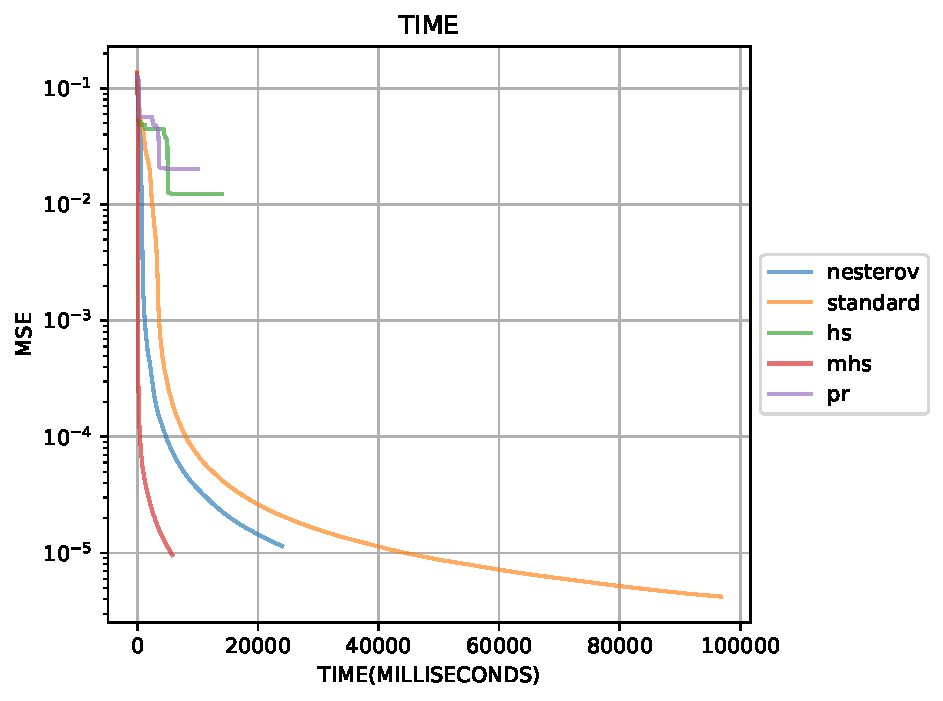
\includegraphics{img/analytics/1_mse_all_time.pdf}
                        }
                        \caption{}
                        \label{fig:monks_1_MSE_all_t}
                    \end{subfigure}
                    \begin{subfigure}{0.45\textwidth}
                        \resizebox{\textwidth}{!}{
                            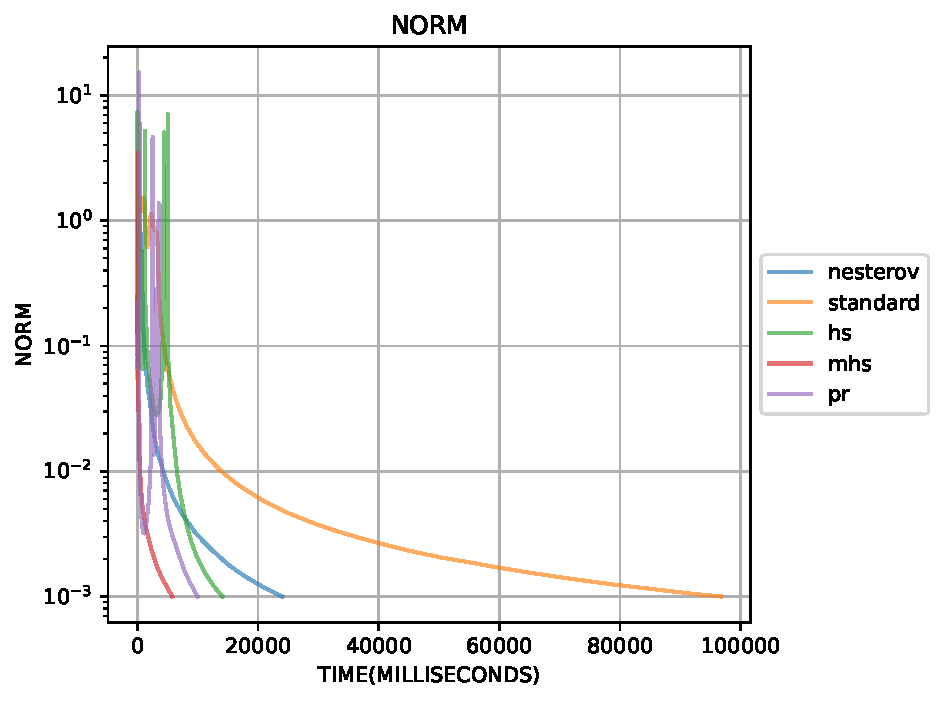
\includegraphics{img/analytics/1_norm_all_time.pdf}
                        }
                        \caption{}
                        \label{fig:monks_1_MSE_all}
                    \end{subfigure}
                    \begin{subfigure}{0.45\textwidth}
                        \resizebox{\textwidth}{!}{
                            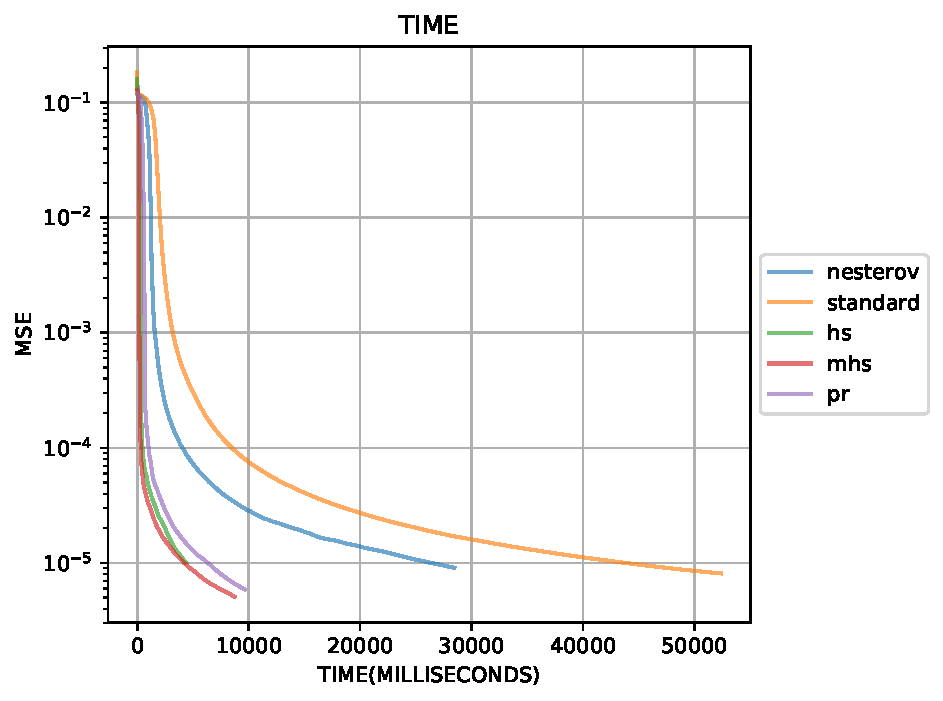
\includegraphics{img/analytics/2_mse_all_time.pdf}
                        }
                        \caption{}
                        \label{fig:monks_2_MSE_all_t}
                    \end{subfigure}
                    \begin{subfigure}{0.45\textwidth}
                        \resizebox{\textwidth}{!}{
                            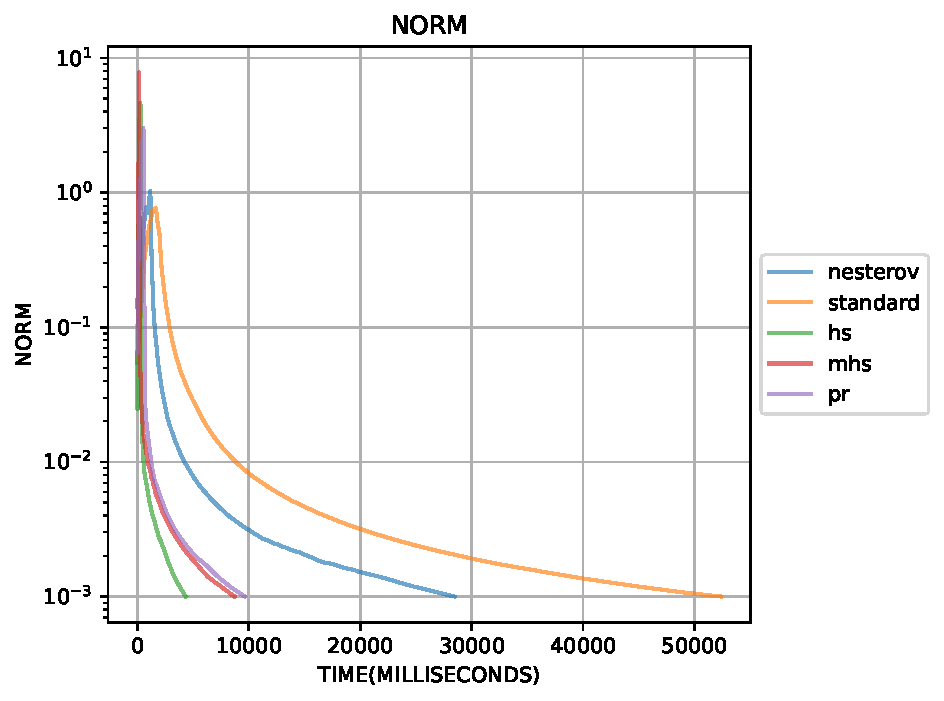
\includegraphics{img/analytics/2_norm_all_time.pdf}
                        }
                        \caption{}
                        \label{fig:monks_2_MSE_all}
                    \end{subfigure}
                    \begin{subfigure}{0.45\textwidth}
                        \resizebox{\textwidth}{!}{
                            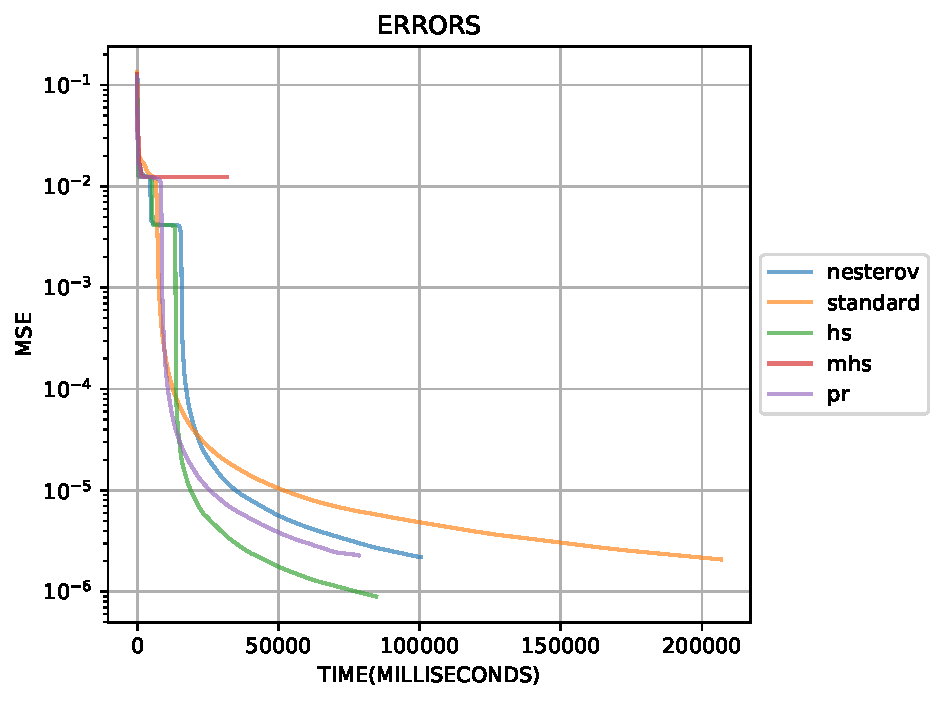
\includegraphics{img/analytics/3_mse_all_time.pdf}
                        }
                        \caption{}
                        \label{fig:monks_3_MSE_all_t}
                    \end{subfigure}
                    \begin{subfigure}{0.45\textwidth}
                        \resizebox{\textwidth}{!}{
                            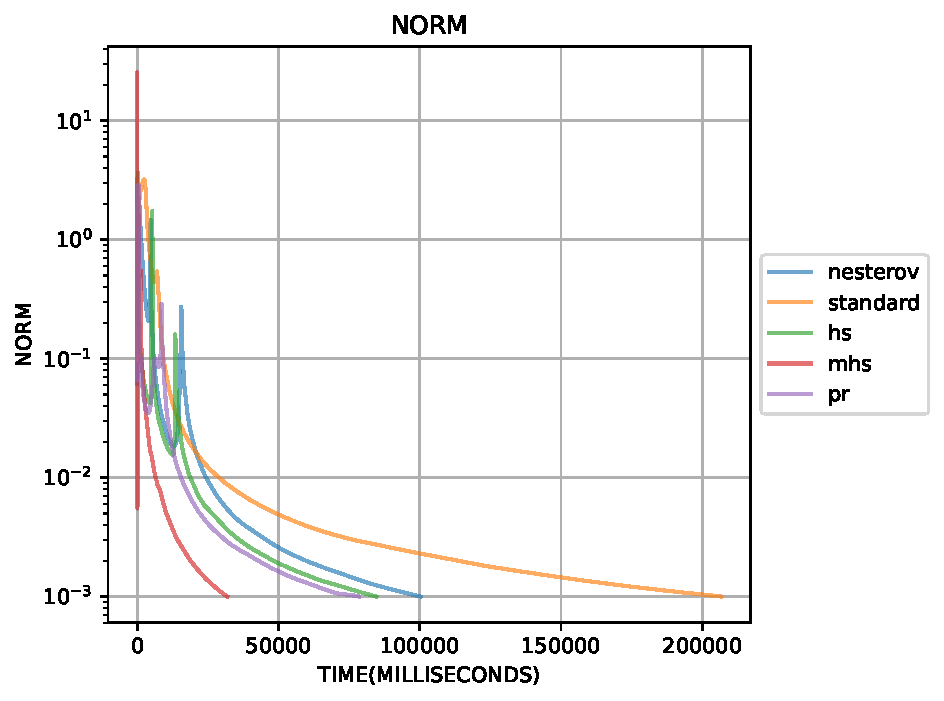
\includegraphics{img/analytics/3_norm_all_time.pdf}
                        }
                        \caption{}
                        \label{fig:monks_3_MSE_all}
                    \end{subfigure}
                    \caption{Comparisons between convergence norm and error of the different optimizers without the constrain of setting a maximal
                    number of epochs for the iterations. In Figure \ref{fig:monks_1_MSE_all}, \ref{fig:monks_1_MSE_all_t} we can see the
                    comparison for MONKS 1, while in Figure \ref{fig:monks_2_MSE_all}, \ref{fig:monks_2_MSE_all_t} we can see the one for
                    MONKS 2 and finally in Figure \ref{fig:monks_3_MSE_all},  \ref{fig:monks_3_MSE_all_t} we can see the one for MONKS 3.}
                    \label{fig:monks_all}
                \end{figure}
       
            \clearpage
            \subsection{Max Epochs 1000}

                \begin{figure}[b!]
                \centering
                \begin{subfigure}{0.45\textwidth}
                    \resizebox{\textwidth}{!}{
                        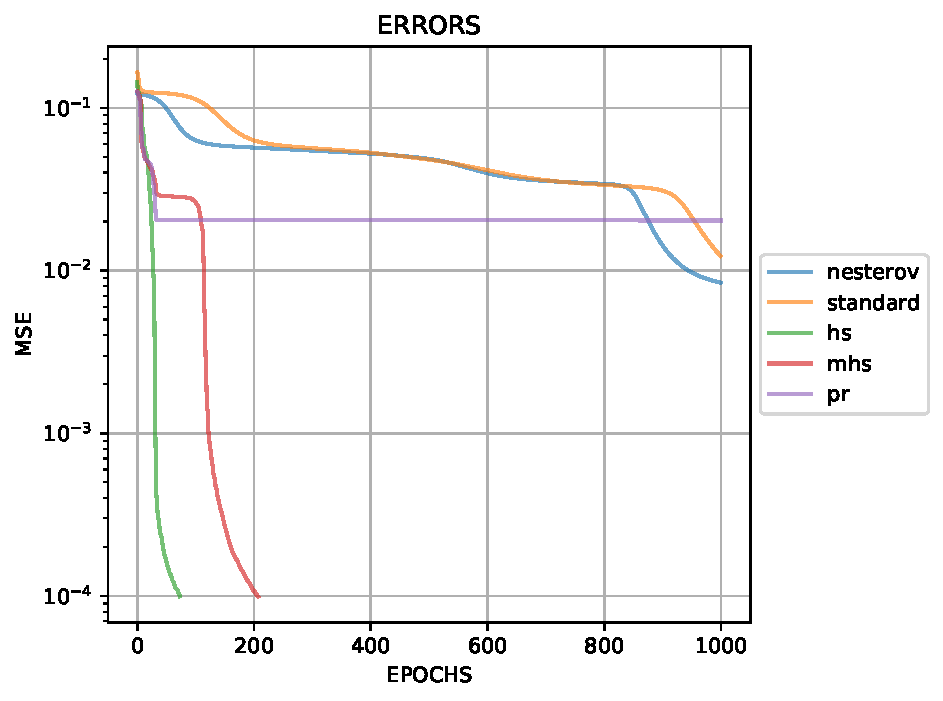
\includegraphics{img/comparisons/1_mse_all_max_epochs_1000.pdf}
                    }
                    \caption{}
                    \label{fig:monks_1_MSE_all_max_epochs_t}
                \end{subfigure}
                \begin{subfigure}{0.45\textwidth}
                    \resizebox{\textwidth}{!}{
                        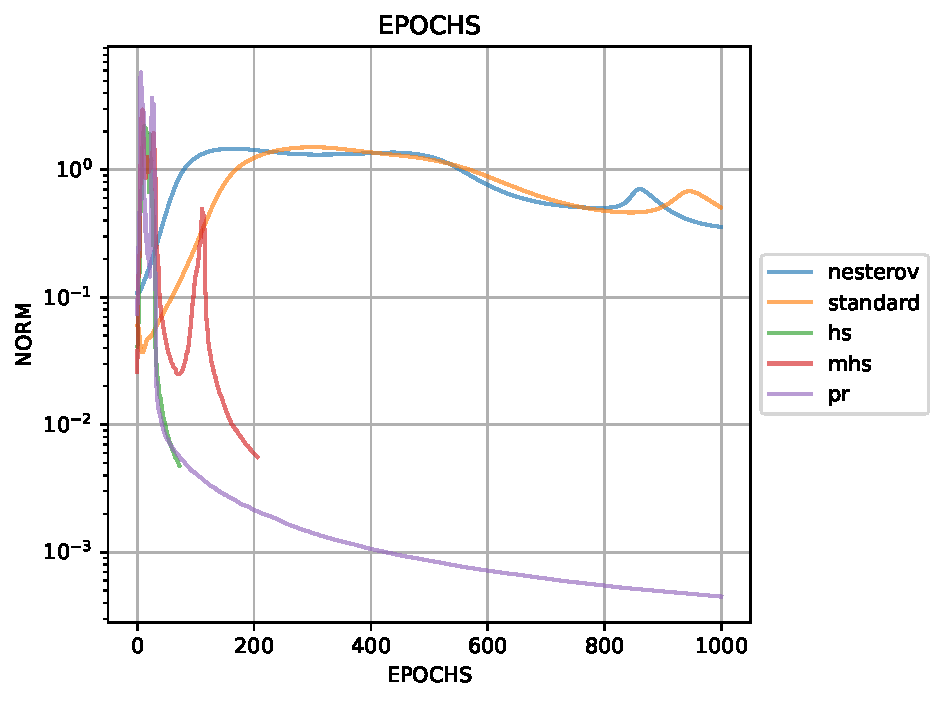
\includegraphics{img/comparisons/1_norm_all_max_epochs_1000.pdf}
                    }
                    \caption{}
                    \label{fig:monks_1_MSE_all_max_epochs}
                \end{subfigure}
                \begin{subfigure}{0.45\textwidth}
                    \resizebox{\textwidth}{!}{
                        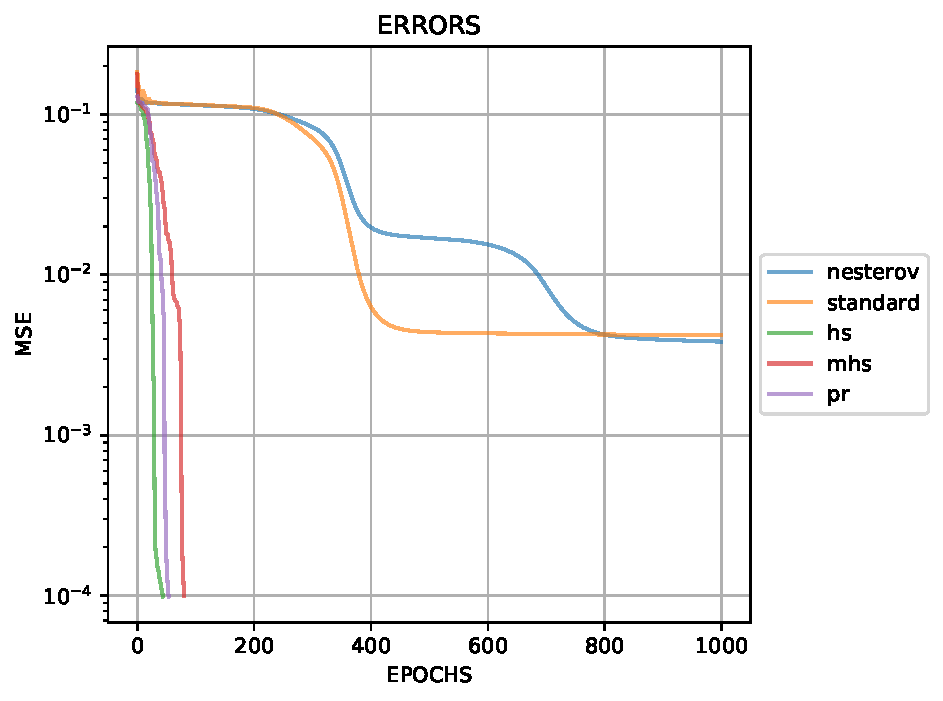
\includegraphics{img/comparisons/2_mse_all_max_epochs_1000.pdf}
                    }
                    \caption{}
                    \label{fig:monks_2_MSE_all_max_epochs_t}
                \end{subfigure}
                \begin{subfigure}{0.45\textwidth}
                    \resizebox{\textwidth}{!}{
                        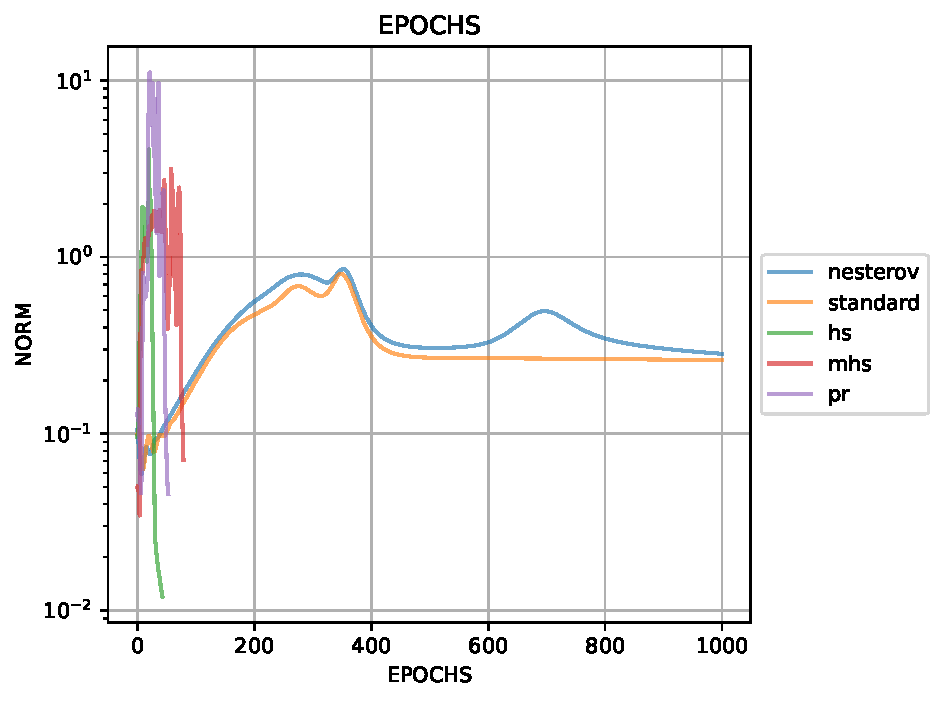
\includegraphics{img/comparisons/2_norm_all_max_epochs_1000.pdf}
                    }
                    \caption{}
                    \label{fig:monks_2_MSE_all_max_epochs}
                \end{subfigure}
                \begin{subfigure}{0.45\textwidth}
                    \resizebox{\textwidth}{!}{
                        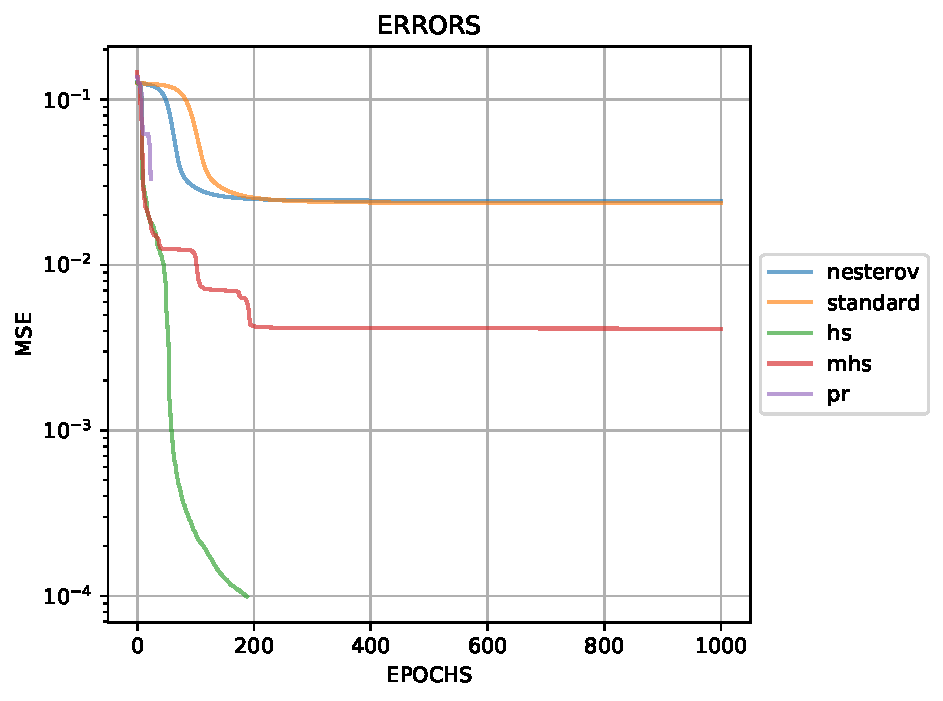
\includegraphics{img/comparisons/3_mse_all_max_epochs_1000.pdf}
                    }
                    \caption{}
                    \label{fig:monks_3_MSE_all_max_epochs_t}
                \end{subfigure}
                \begin{subfigure}{0.45\textwidth}
                    \resizebox{\textwidth}{!}{
                        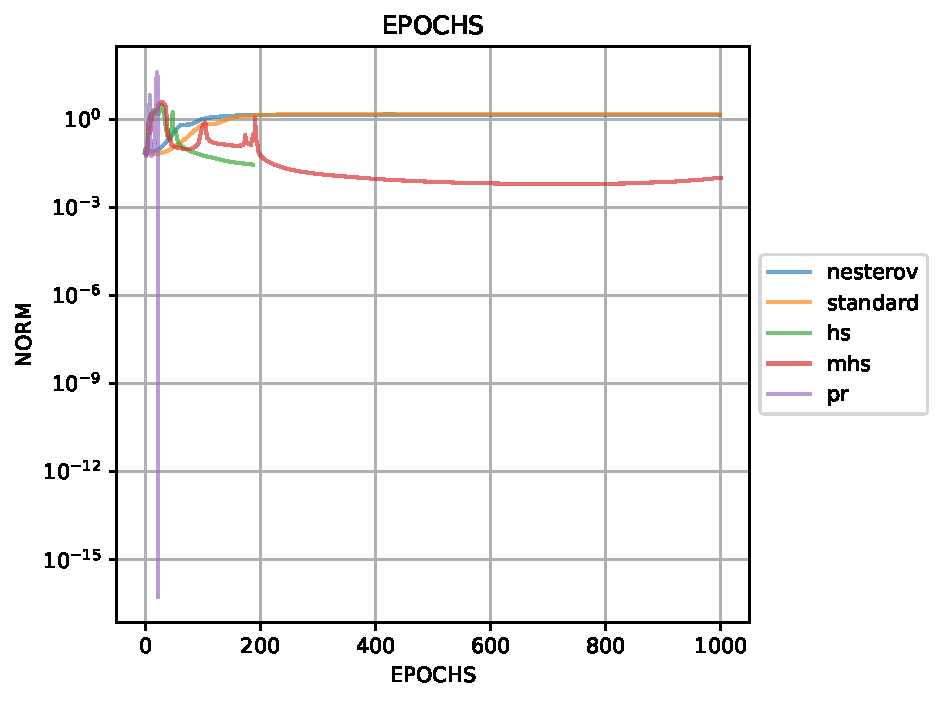
\includegraphics{img/comparisons/3_norm_all_max_epochs_1000.pdf}
                    }
                    \caption{}
                    \label{fig:monks_3_MSE_all_max_epochs}
                \end{subfigure}
                \caption{Comparisons between convergence norm and error the different optimizers with the constrain of setting a
                maximal number of epochs egual to 1000. In Figure \ref{fig:monks_1_MSE_all_max_epochs}, \ref{fig:monks_1_MSE_all_max_epochs_t}
                we can see the comparison for MONKS 1, while in Figure \ref{fig:monks_2_MSE_all_max_epochs}, \ref{fig:monks_2_MSE_all_max_epochs_t}
                we can see the one for MONKS 2 and finally in Figure \ref{fig:monks_3_MSE_all_max_epochs}, \ref{fig:monks_3_MSE_all_max_epochs_t} we
                can see the one for MONKS 3.}
                \label{fig:monks_MSE_all_max_epochs}
            \end{figure}


        \clearpage
        \section{Stochastic Gradient Descent} % (fold)
        \label{sec:stochastic_gradient_descent}
            
            \subsection{No Max Epochs}

            \begin{figure}[H]
                \centering
                \begin{subfigure}{0.40\textwidth}
                    \resizebox{\textwidth}{!}{
                        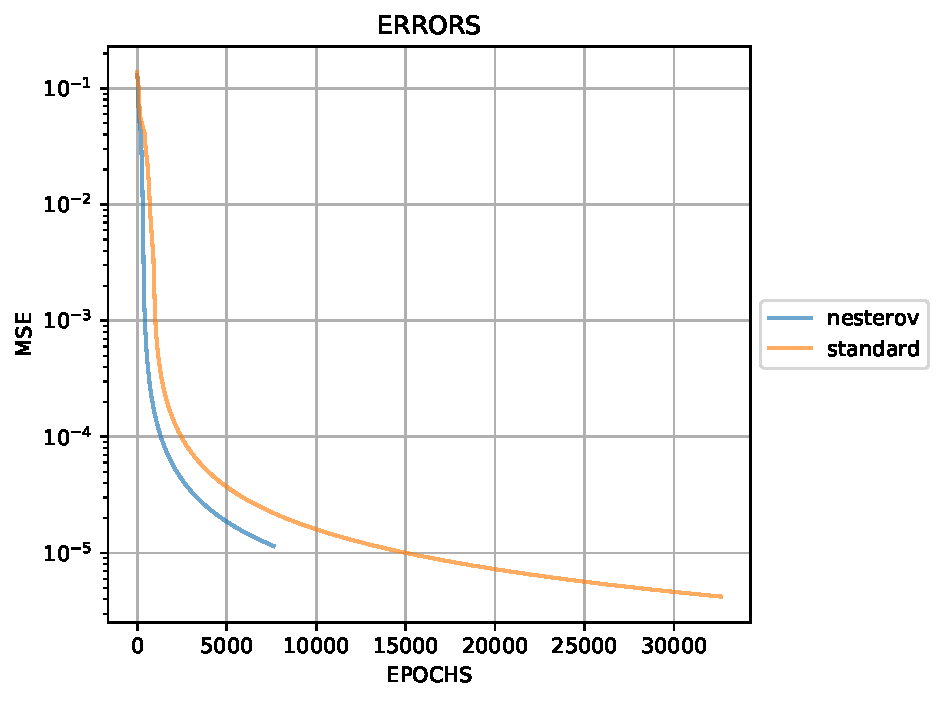
\includegraphics{img/analytics/1_mse_momentum.pdf}
                    }
                    \caption{}
                    \label{fig:monks_1_MSE_SGD}
                \end{subfigure}
                \begin{subfigure}{0.40\textwidth}
                    \resizebox{\textwidth}{!}{
                        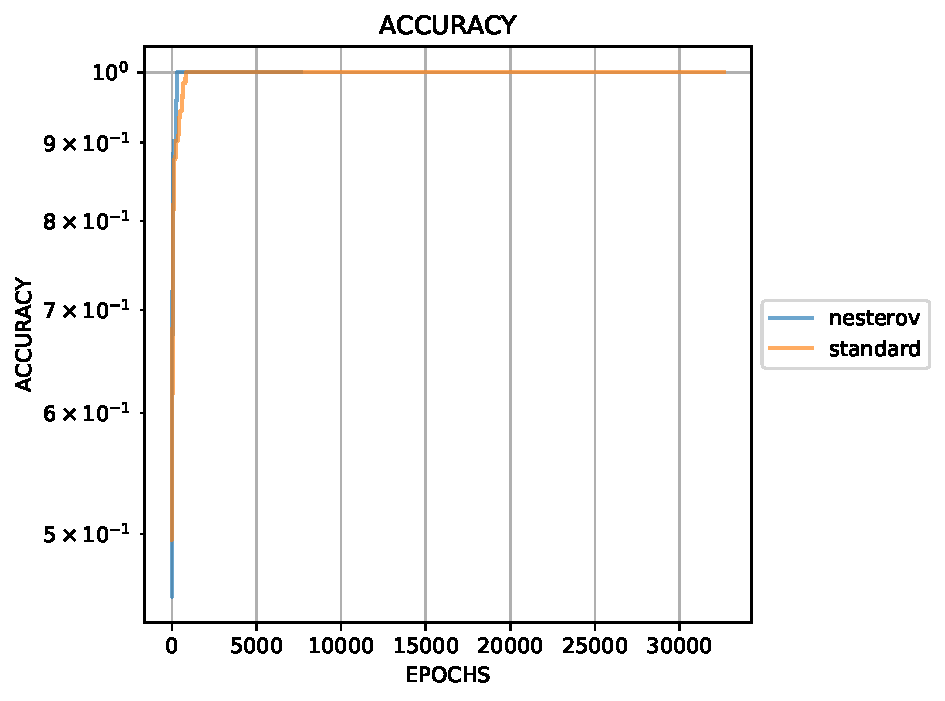
\includegraphics{img/analytics/1_accuracy_momentum.pdf}
                    }
                    \caption{}
                    \label{fig:monks_1_ACC_SGD}
                \end{subfigure}
                \begin{subfigure}{0.40\textwidth}
                    \resizebox{\textwidth}{!}{
                        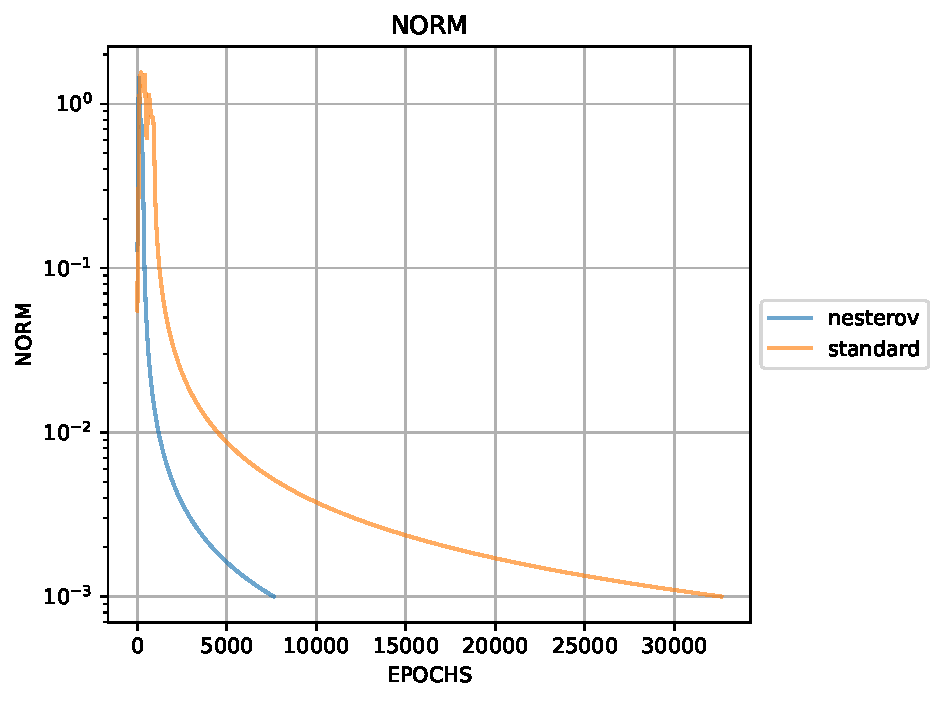
\includegraphics{img/analytics/1_norm_momentum.pdf}
                    }
                    \caption{}
                    \label{fig:monks_1_NORM_SGD}
                \end{subfigure}
                \caption{Example of a final learning, accuracy score and convergence of norm curve on MONKS 1 with standard and nesterov momentum.}
                \label{fig:monks_1_SGD}
            \end{figure}

             \begin{figure}[H]
                \centering
                \begin{subfigure}{0.40\textwidth}
                    \resizebox{\textwidth}{!}{
                        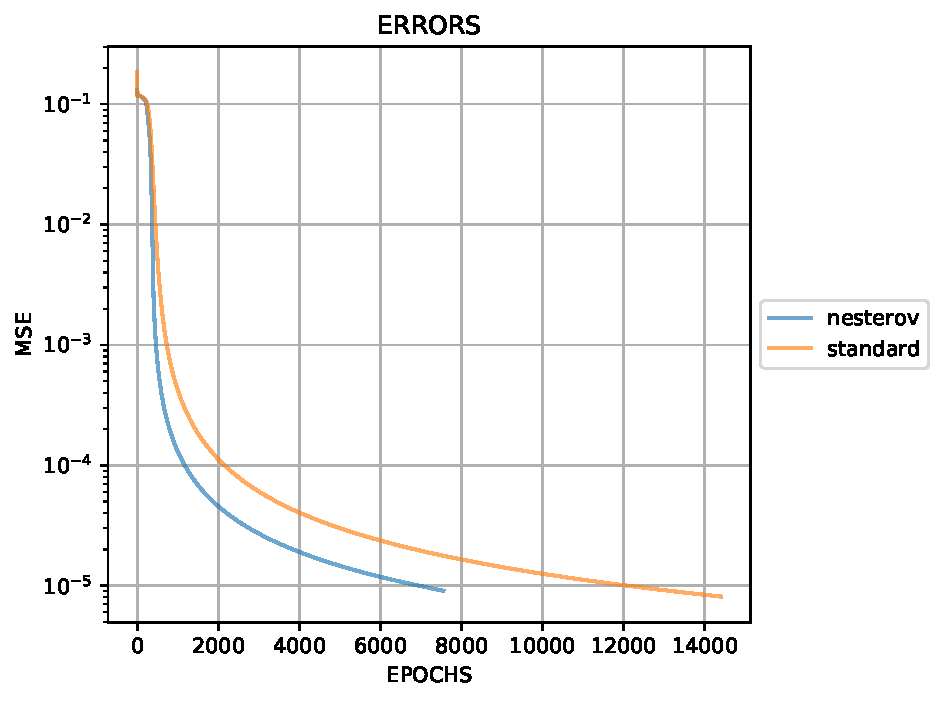
\includegraphics{img/analytics/2_mse_momentum.pdf}
                    }
                    \caption{}
                    \label{fig:monks_2_MSE_SGD}
                \end{subfigure}
                \begin{subfigure}{0.40\textwidth}
                    \resizebox{\textwidth}{!}{
                        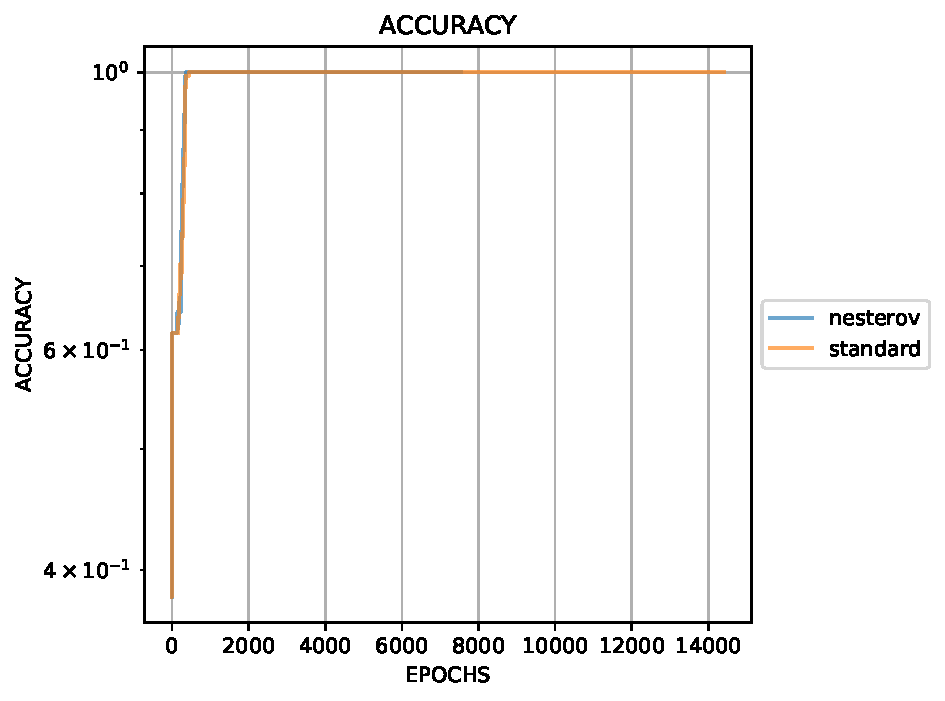
\includegraphics{img/analytics/2_accuracy_momentum.pdf}
                    }
                    \caption{}
                    \label{fig:monks_2_ACC_SGD}
                \end{subfigure}
                \begin{subfigure}{0.40\textwidth}
                    \resizebox{\textwidth}{!}{
                        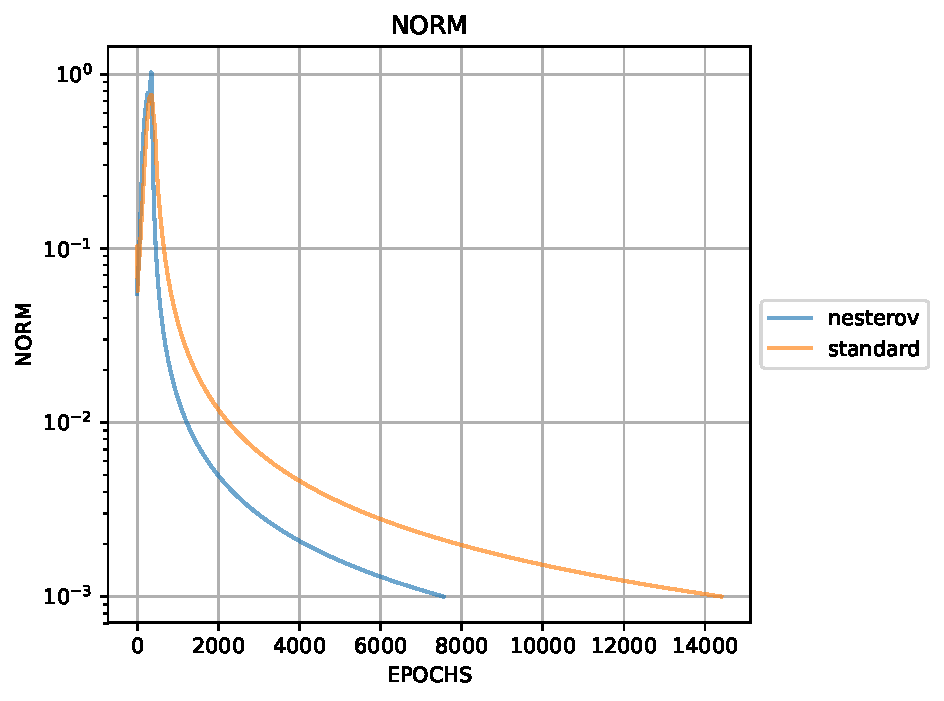
\includegraphics{img/analytics/2_norm_momentum.pdf}
                    }
                    \caption{}
                    \label{fig:monks_2_NORM_SGD}
                \end{subfigure}
                \caption{Example of a final learning, accuracy score and convergence of norm curve on MONKS 2 with standard and nesterov momentum.}
                \label{fig:monks_2_SGD}
            \end{figure}

            \begin{figure}[H]
                \centering
                \begin{subfigure}{0.40\textwidth}
                    \resizebox{\textwidth}{!}{
                        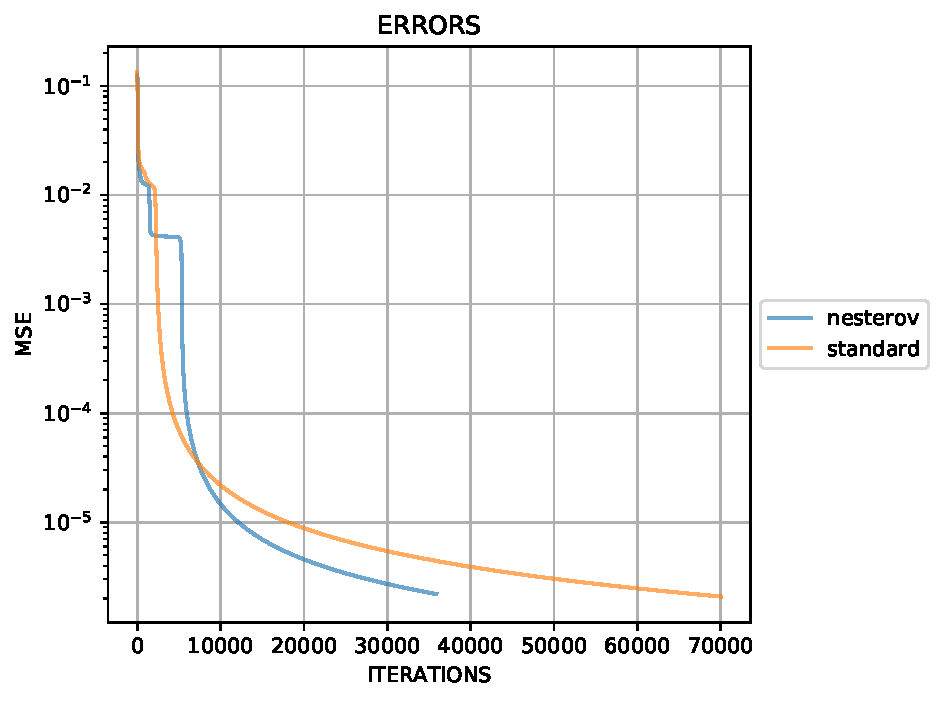
\includegraphics{img/analytics/3_mse_momentum.pdf}
                    }
                    \caption{}
                    \label{fig:monks_3_MSE_SGD}
                \end{subfigure}
                \begin{subfigure}{0.40\textwidth}
                    \resizebox{\textwidth}{!}{
                        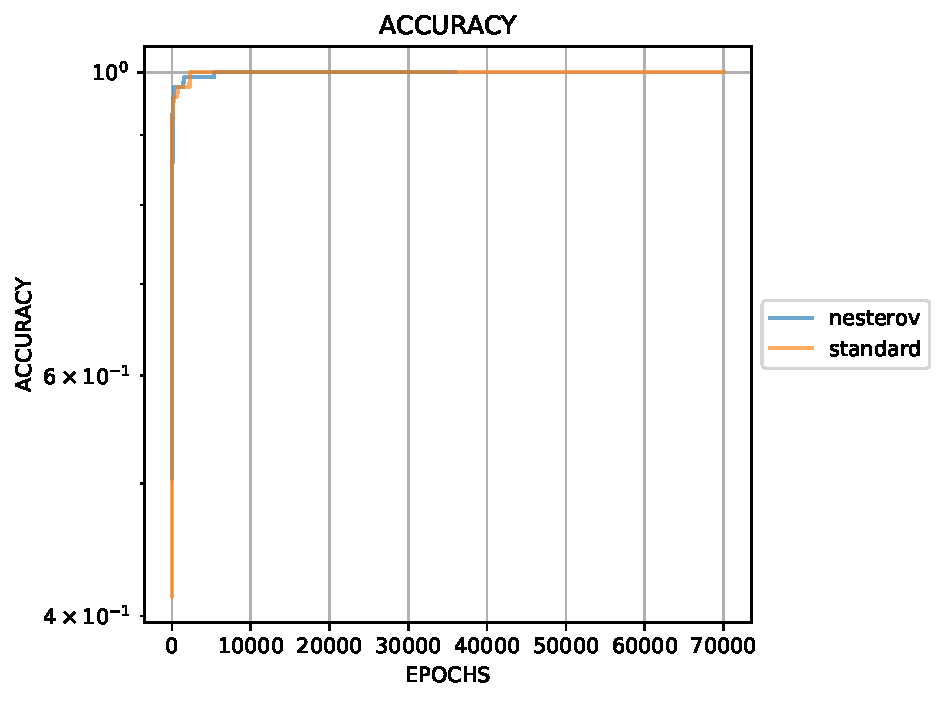
\includegraphics{img/analytics/3_accuracy_momentum.pdf}
                    }
                    \caption{}
                    \label{fig:monks_3_ACC_SGD}
                \end{subfigure}
                \begin{subfigure}{0.40\textwidth}
                    \resizebox{\textwidth}{!}{
                        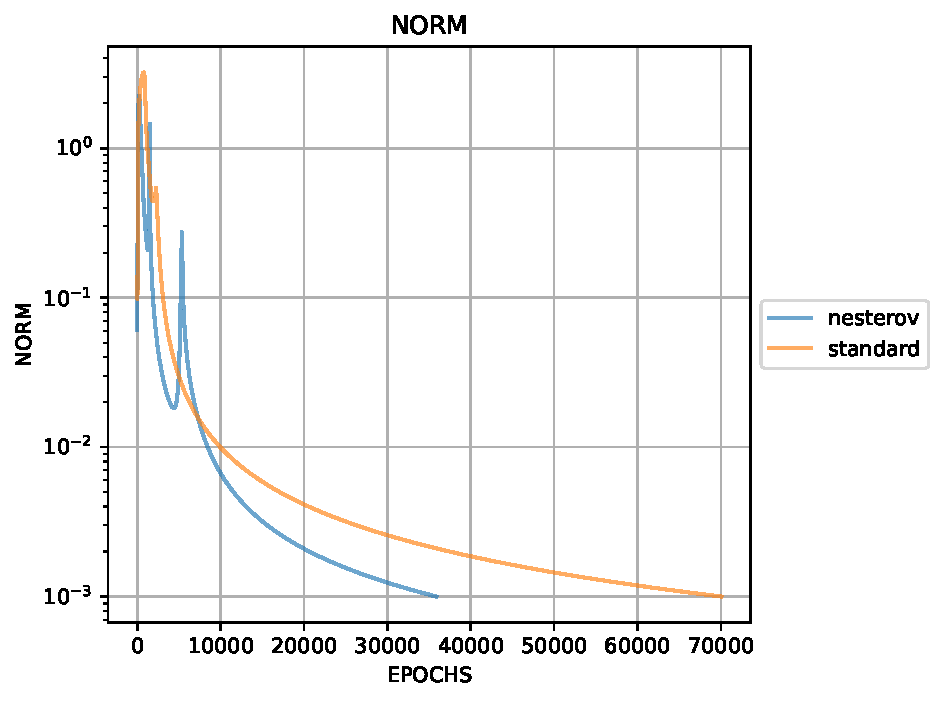
\includegraphics{img/analytics/3_norm_momentum.pdf}
                    }
                    \caption{}
                    \label{fig:monks_3_NORM_SGD}
                \end{subfigure}
                \caption{Example of a final learning, accuracy score and convergence of norm curve on MONKS 3 with standard and nesterov momentum.}
                \label{fig:monks_3_SGD}
            \end{figure}

            \subsection{Max Epochs 1000}

            \begin{figure}[H]
                \centering
                \begin{subfigure}{0.40\textwidth}
                    \resizebox{\textwidth}{!}{
                        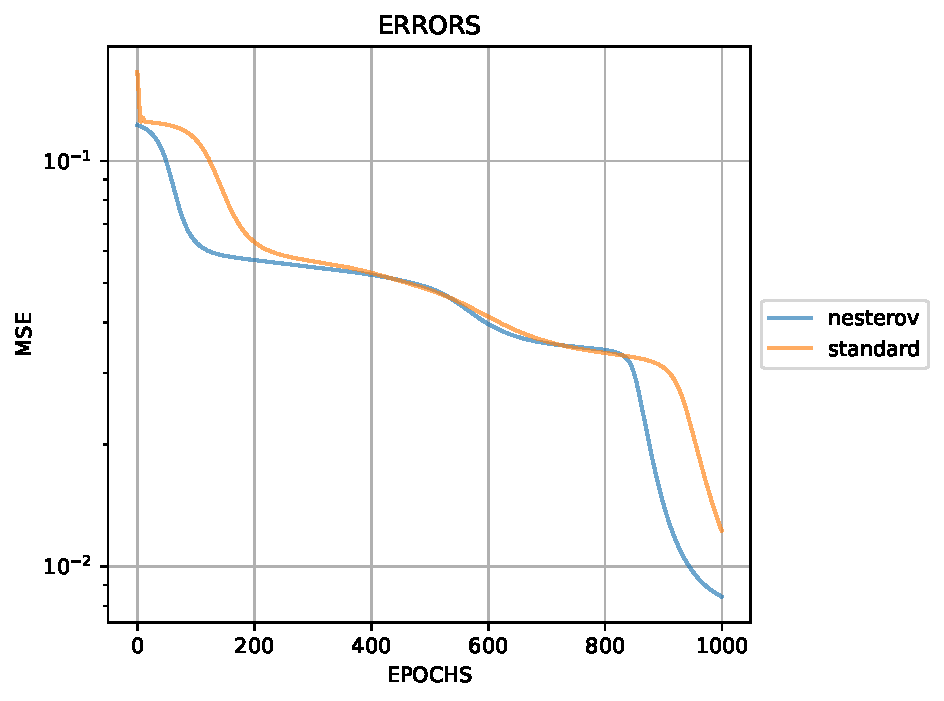
\includegraphics{img/comparisons/1_mse_momentum_max_epochs_1000.pdf}
                    }
                    \caption{}
                    \label{fig:monks_1_MSE_SGD}
                \end{subfigure}
                \begin{subfigure}{0.40\textwidth}
                    \resizebox{\textwidth}{!}{
                        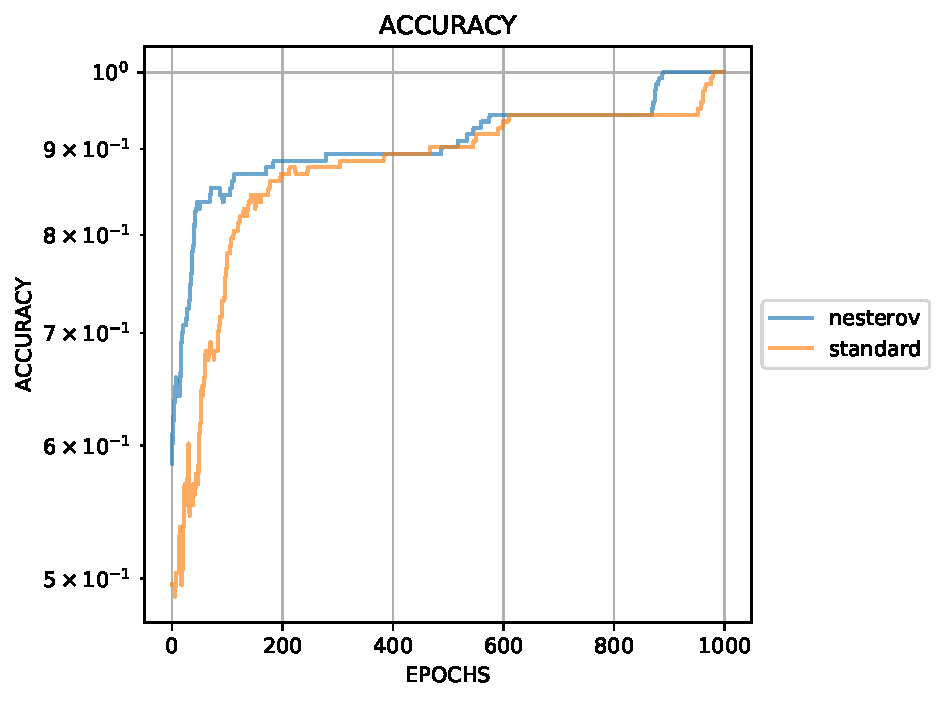
\includegraphics{img/comparisons/1_accuracy_momentum_max_epochs_1000.pdf}
                    }
                    \caption{}
                    \label{fig:monks_1_ACC_SGD}
                \end{subfigure}
                \begin{subfigure}{0.40\textwidth}
                    \resizebox{\textwidth}{!}{
                        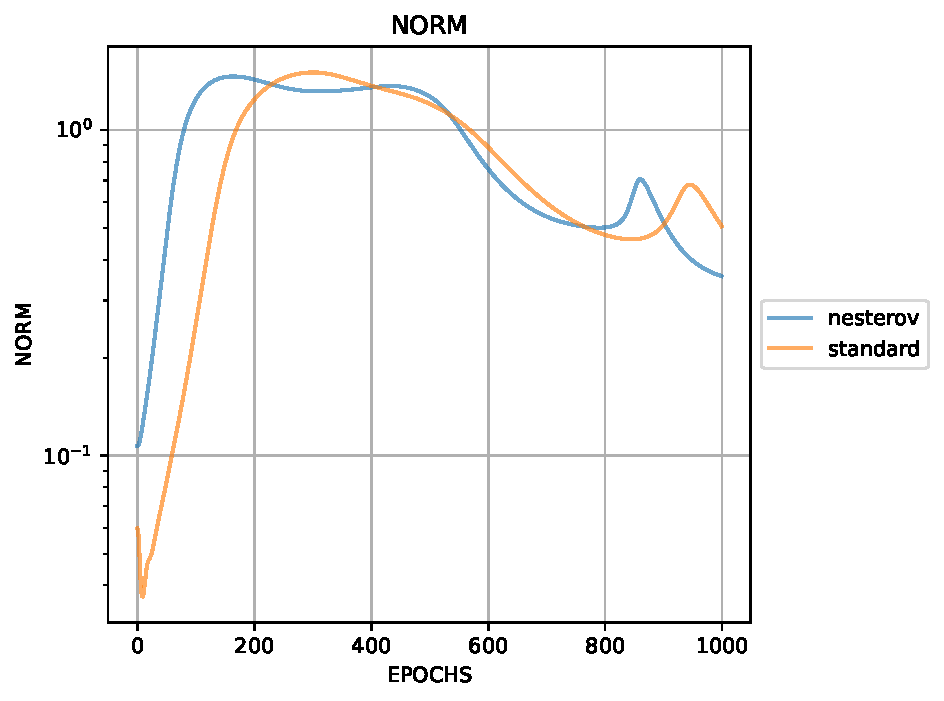
\includegraphics{img/comparisons/1_norm_momentum_max_epochs_1000.pdf}
                    }
                    \caption{}
                    \label{fig:monks_1_NORM_SGD}
                \end{subfigure}
                \caption{Example of a final learning, accuracy score and convergence of norm curve on MONKS 1 with standard and nesterov momentum.}
                \label{fig:monks_1_SGD}
            \end{figure}

             \begin{figure}[H]
                \centering
                \begin{subfigure}{0.40\textwidth}
                    \resizebox{\textwidth}{!}{
                        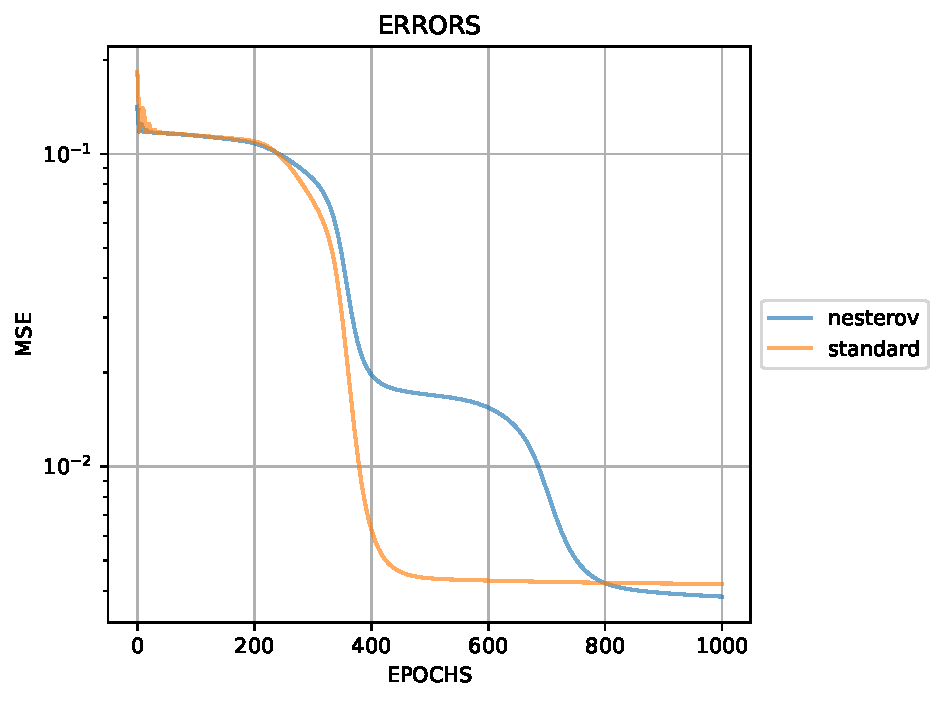
\includegraphics{img/comparisons/2_mse_momentum_max_epochs_1000.pdf}
                    }
                    \caption{}
                    \label{fig:monks_2_MSE_SGD}
                \end{subfigure}
                \begin{subfigure}{0.40\textwidth}
                    \resizebox{\textwidth}{!}{
                        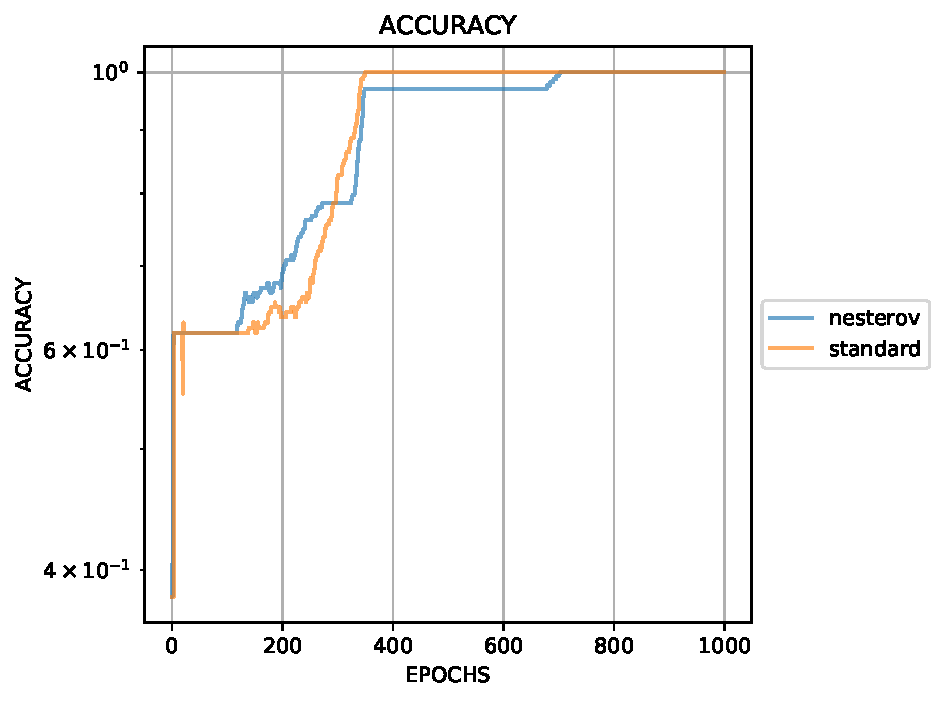
\includegraphics{img/comparisons/2_accuracy_momentum_max_epochs_1000.pdf}
                    }
                    \caption{}
                    \label{fig:monks_2_ACC_SGD}
                \end{subfigure}
                \begin{subfigure}{0.40\textwidth}
                    \resizebox{\textwidth}{!}{
                        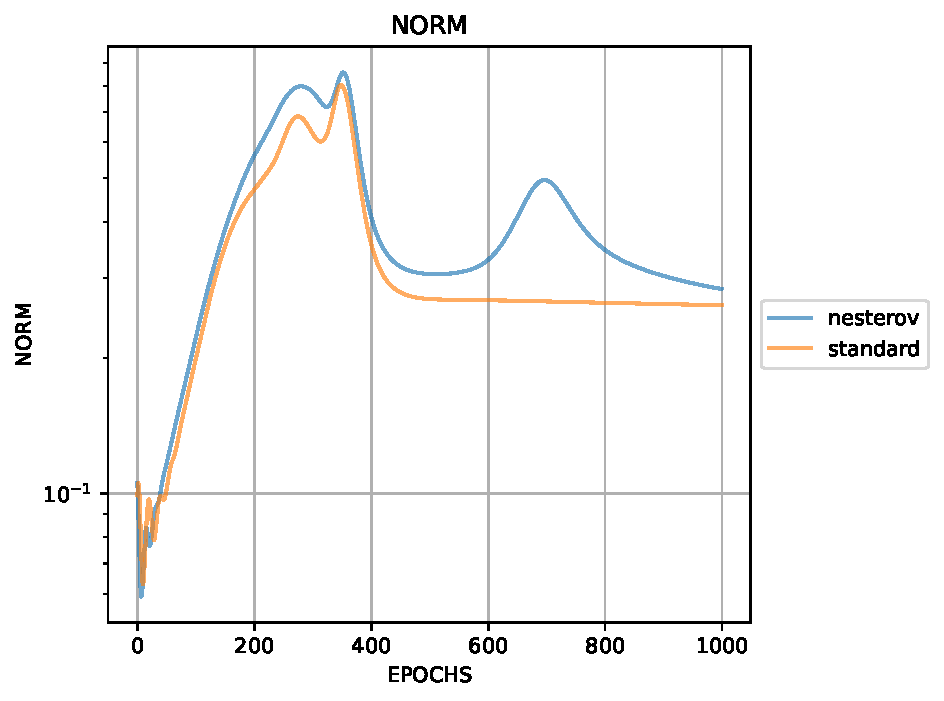
\includegraphics{img/comparisons/2_norm_momentum_max_epochs_1000.pdf}
                    }
                    \caption{}
                    \label{fig:monks_2_NORM_SGD}
                \end{subfigure}
                \caption{Example of a final learning, accuracy score and convergence of norm curve on MONKS 2 with standard and nesterov momentum.}
                \label{fig:monks_2_SGD}
            \end{figure}

            \begin{figure}[H]
                \centering
                \begin{subfigure}{0.40\textwidth}
                    \resizebox{\textwidth}{!}{
                        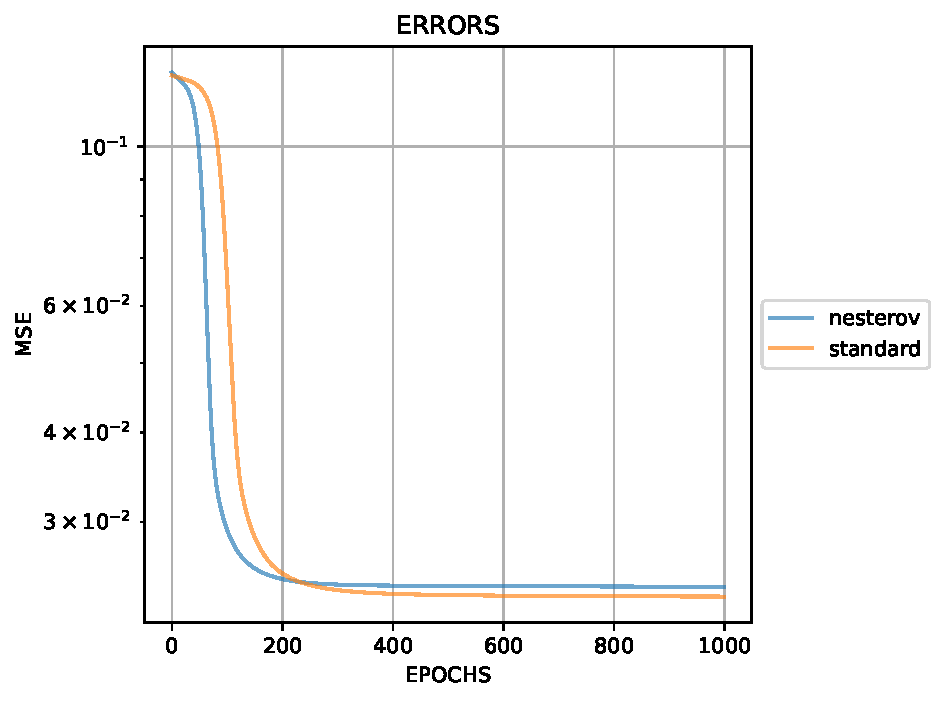
\includegraphics{img/comparisons/3_mse_momentum_max_epochs_1000.pdf}
                    }
                    \caption{}
                    \label{fig:monks_3_MSE_SGD}
                \end{subfigure}
                \begin{subfigure}{0.40\textwidth}
                    \resizebox{\textwidth}{!}{
                        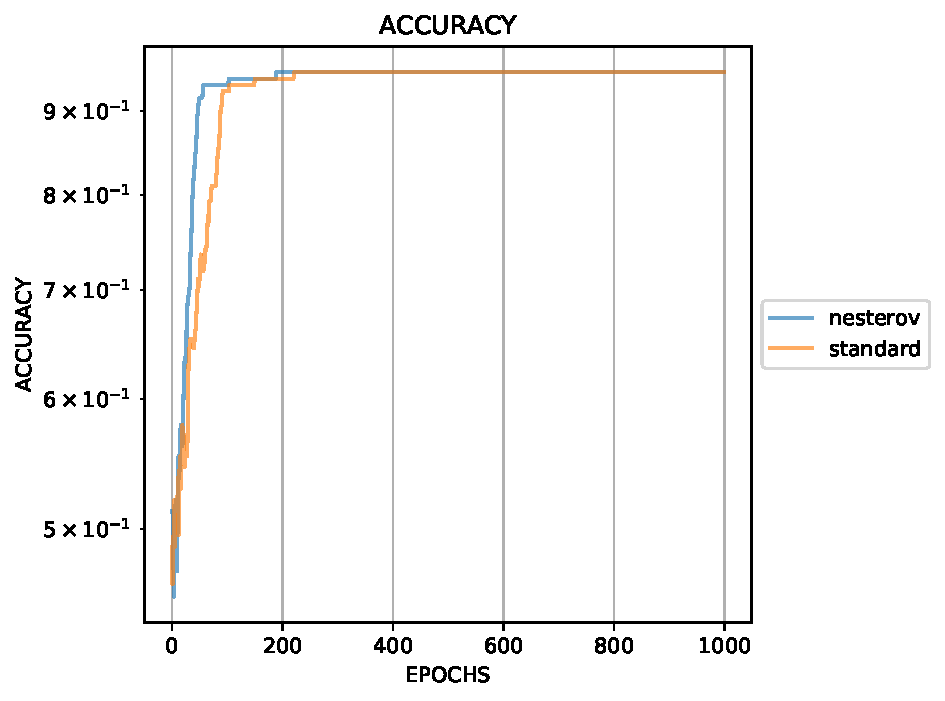
\includegraphics{img/comparisons/3_accuracy_momentum_max_epochs_1000.pdf}
                    }
                    \caption{}
                    \label{fig:monks_3_ACC_SGD}
                \end{subfigure}
                \begin{subfigure}{0.40\textwidth}
                    \resizebox{\textwidth}{!}{
                        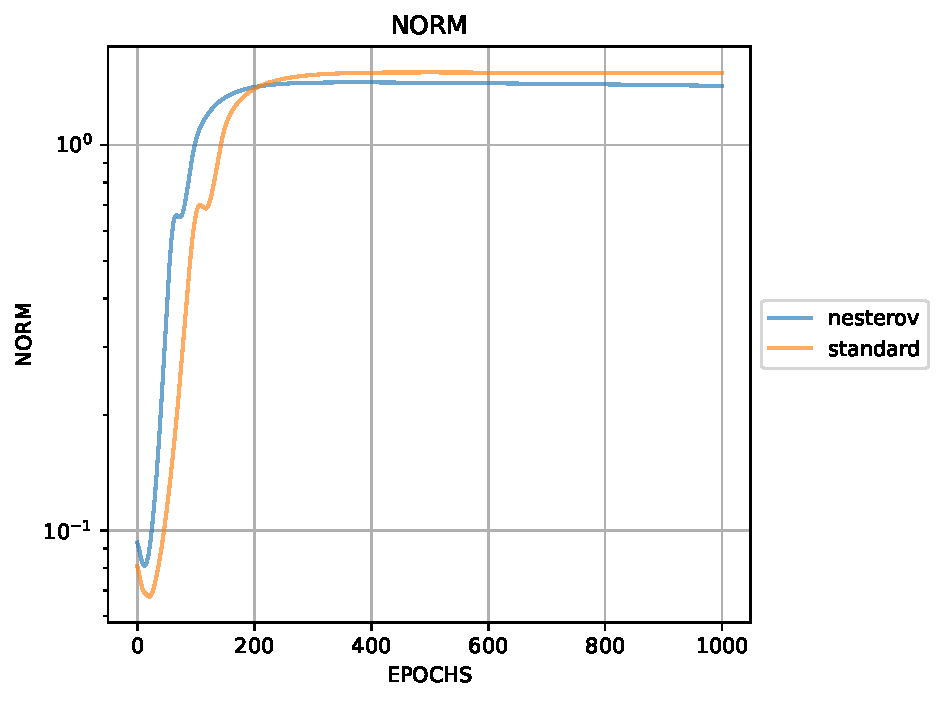
\includegraphics{img/comparisons/3_norm_momentum_max_epochs_1000.pdf}
                    }
                    \caption{}
                    \label{fig:monks_3_NORM_SGD}
                \end{subfigure}
                \caption{Example of a final learning, accuracy score and convergence of norm curve on MONKS 3 with standard and nesterov momentum.}
                \label{fig:monks_3_SGD}
            \end{figure}


         \section{Conjugate Gradient Methods} % (fold)
         \label{sec:conjugate_gradient_methods}
            \subsection{No Max Epochs} % (fold)
            \label{sub:comparisons}

            \begin{figure}[H]
                \centering
                \begin{subfigure}{0.4\textwidth}
                    \resizebox{\textwidth}{!}{
                        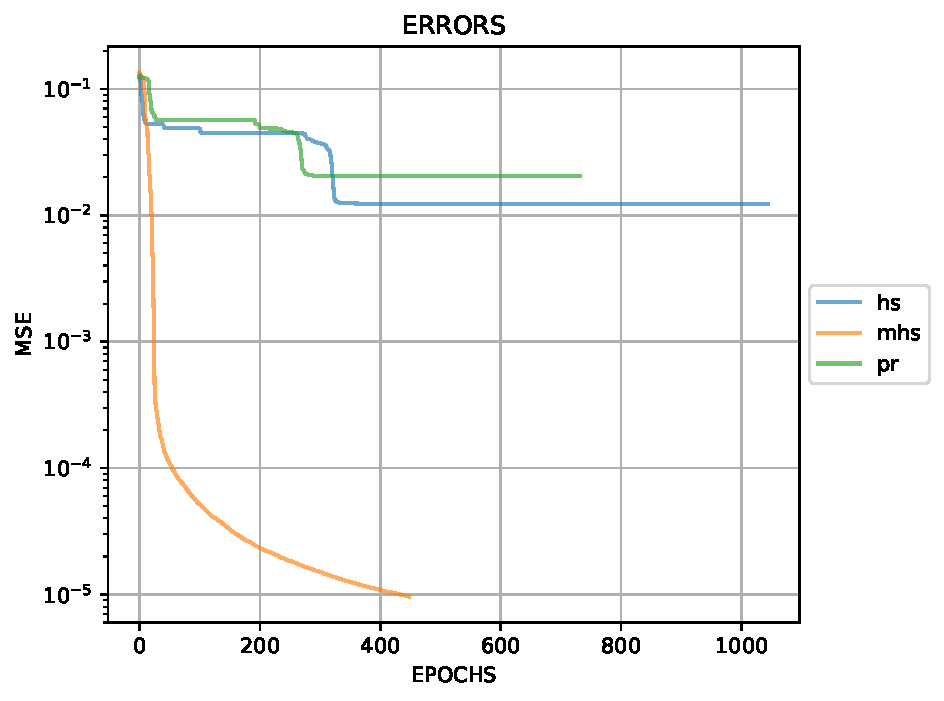
\includegraphics{img/analytics/1_mse_beta.pdf}
                    }
                    \caption{}
                    \label{fig:monks_1_MSE_CGD}
                \end{subfigure}
                \begin{subfigure}{0.4\textwidth}
                    \resizebox{\textwidth}{!}{
                        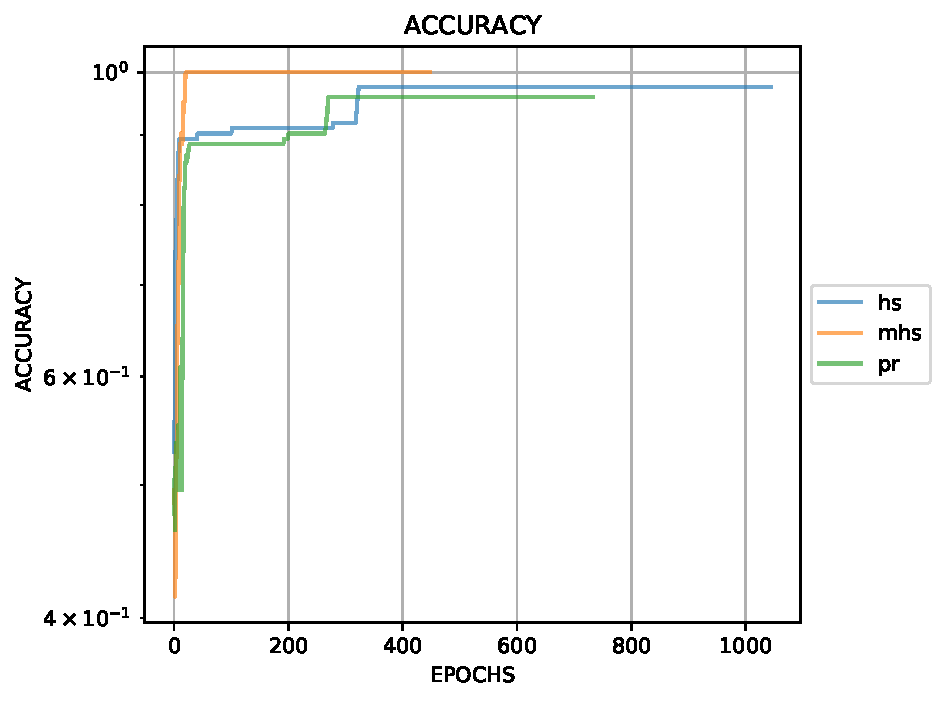
\includegraphics{img/analytics/1_accuracy_beta.pdf}
                    }
                    \caption{}
                    \label{fig:monks_1_ACC_CGD}
                \end{subfigure}
                \begin{subfigure}{0.4\textwidth}
                    \resizebox{\textwidth}{!}{
                        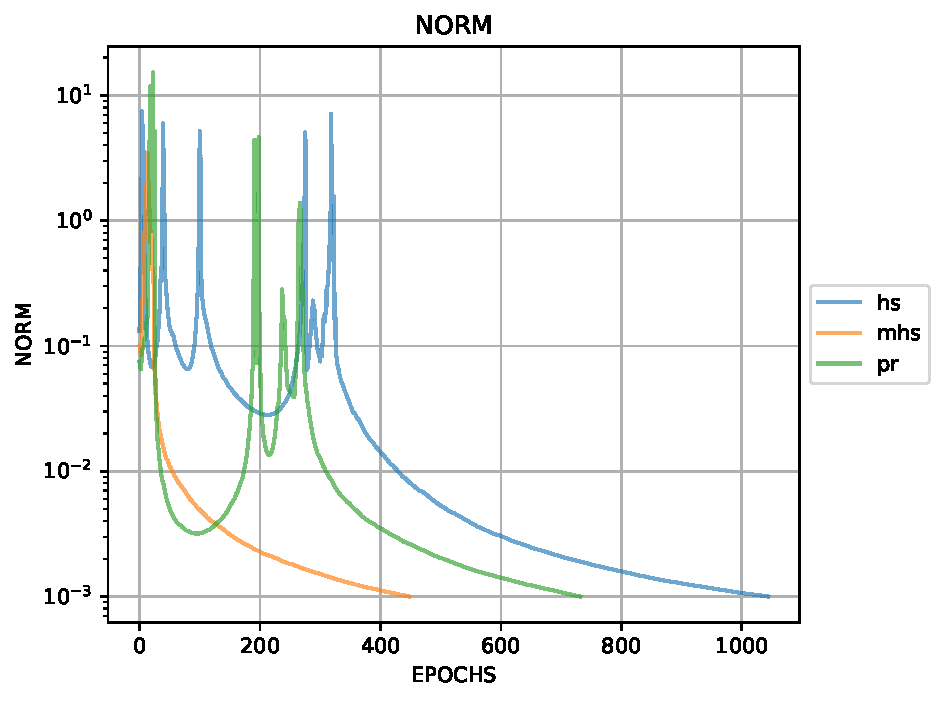
\includegraphics{img/analytics/1_norm_beta.pdf}
                    }
                    \caption{}
                    \label{fig:monks_1_NORM_CGD}
                \end{subfigure}
                \caption{Example of a final learning, accuracy score and convergence of norm curve on MONKS 1 with different beta methods.}
                \label{fig:monks_1_CGD}
            \end{figure}

             \begin{figure}[H]
                \centering
                \begin{subfigure}{0.40\textwidth}
                    \resizebox{\textwidth}{!}{
                        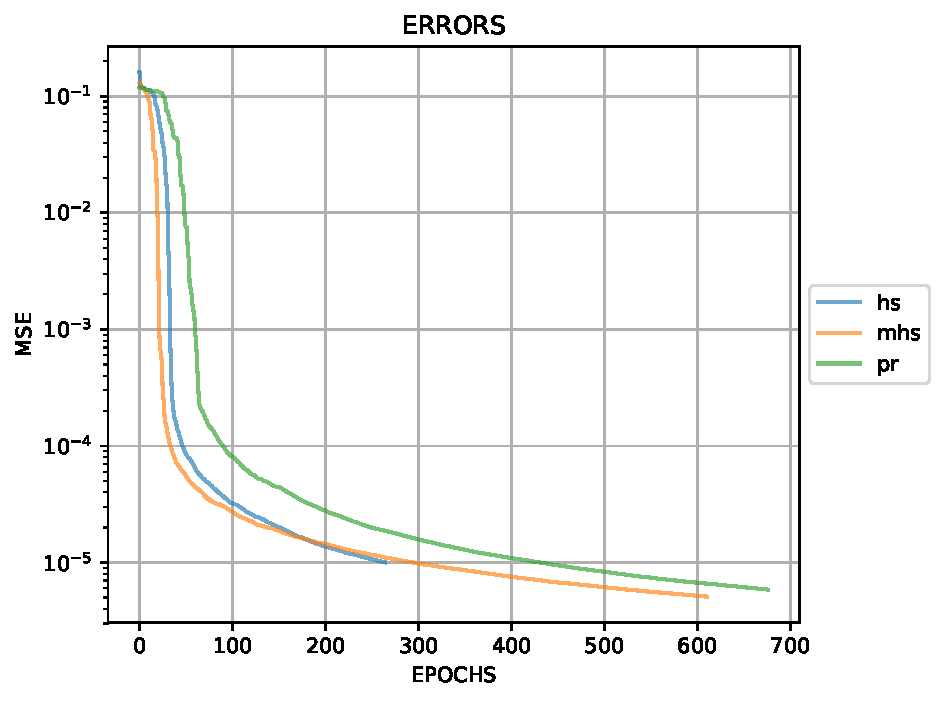
\includegraphics{img/analytics/2_mse_beta.pdf}
                    }
                    \caption{}
                    \label{fig:monks_2_MSE_CGD}
                \end{subfigure}
                \begin{subfigure}{0.40\textwidth}
                    \resizebox{\textwidth}{!}{
                        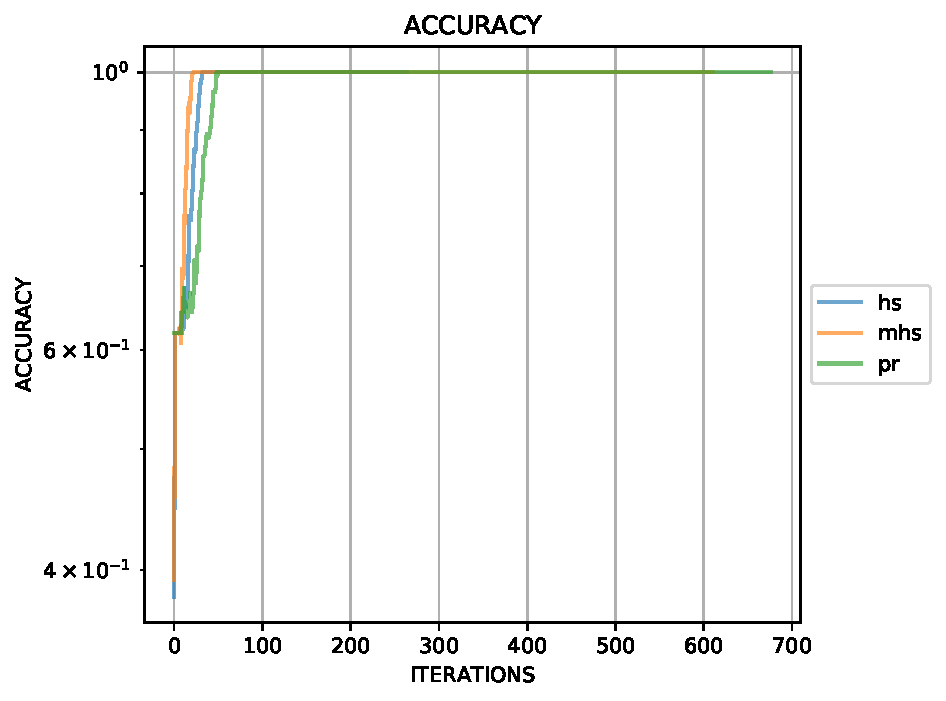
\includegraphics{img/analytics/2_accuracy_beta.pdf}
                    }
                    \caption{}
                    \label{fig:monks_2_ACC_CGD}
                \end{subfigure}
                \begin{subfigure}{0.40\textwidth}
                    \resizebox{\textwidth}{!}{
                        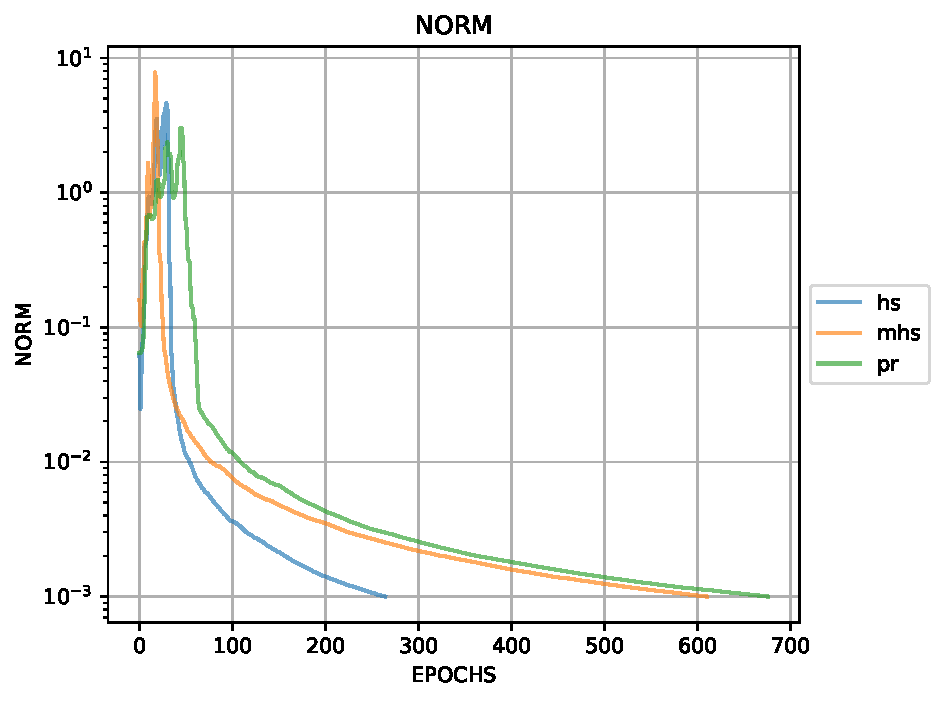
\includegraphics{img/analytics/2_norm_beta.pdf}
                    }
                    \caption{}
                    \label{fig:monks_2_NORM_CGD}
                \end{subfigure}
                \caption{Example of a final learning, accuracy score and convergence of norm curve on MONKS 2 with different beta methods.}
                \label{fig:monks_2_CGD}
            \end{figure}

            \begin{figure}[H]
                \centering
                \begin{subfigure}{0.40\textwidth}
                    \resizebox{\textwidth}{!}{
                        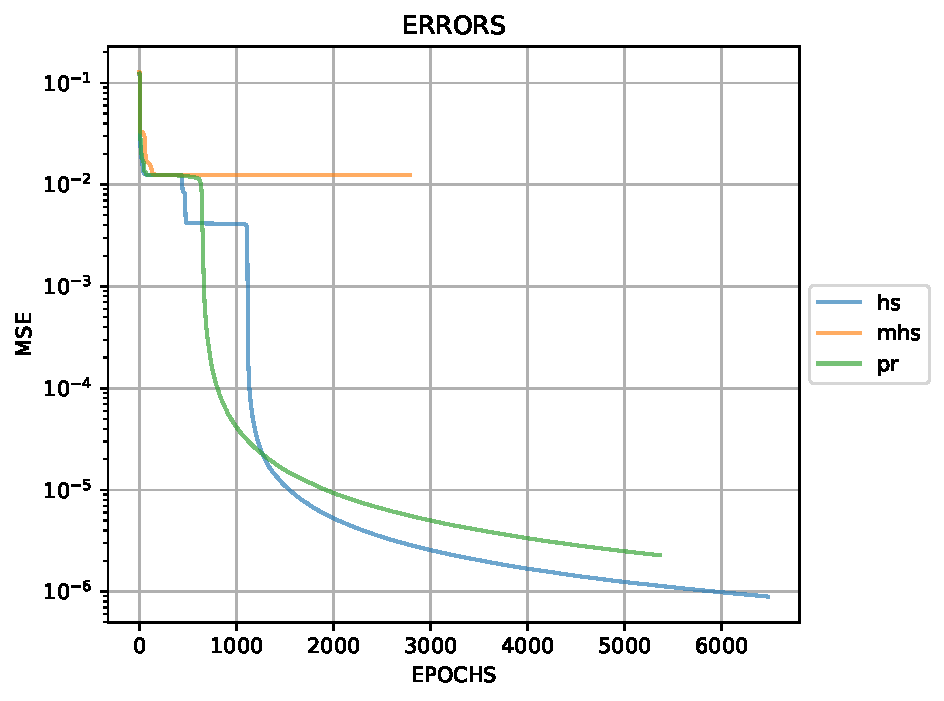
\includegraphics{img/analytics/3_mse_beta.pdf}
                    }
                    \caption{}
                    \label{fig:monks_3_MSE_CGD}
                \end{subfigure}
                \begin{subfigure}{0.40\textwidth}
                    \resizebox{\textwidth}{!}{
                        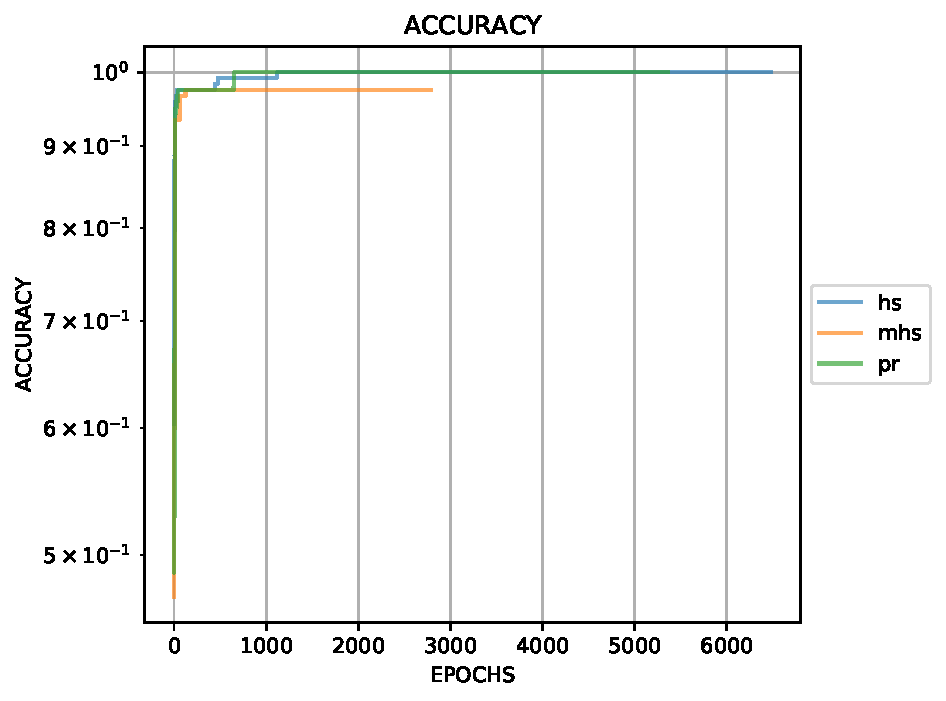
\includegraphics{img/analytics/3_accuracy_beta.pdf}
                    }
                    \caption{}
                    \label{fig:monks_3_ACC_CGD}
                \end{subfigure}
                \begin{subfigure}{0.40\textwidth}
                    \resizebox{\textwidth}{!}{
                        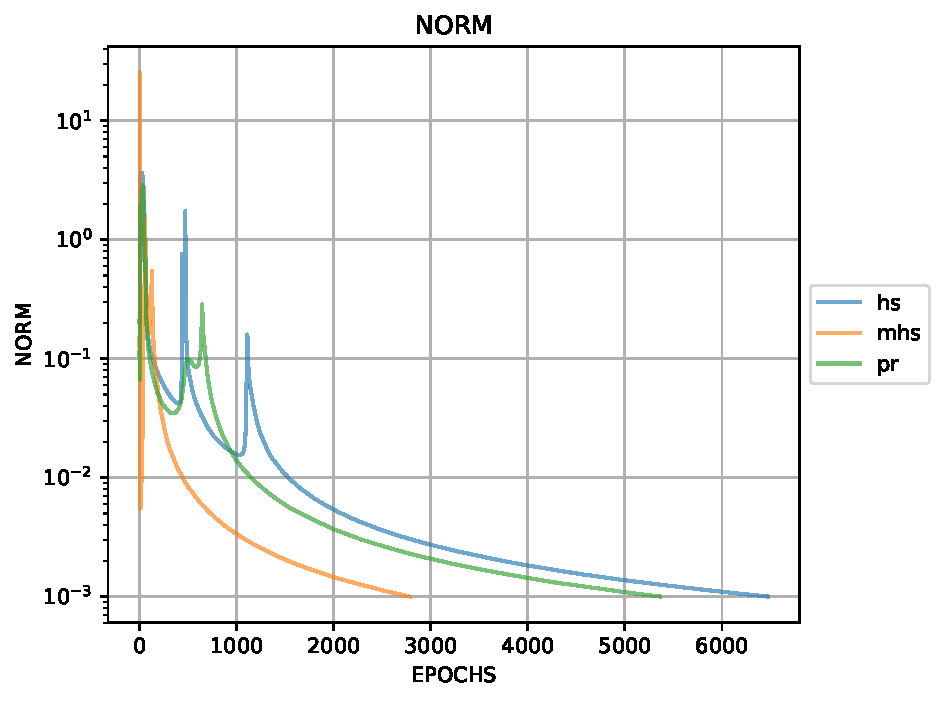
\includegraphics{img/analytics/3_norm_beta.pdf}
                    }
                    \caption{}
                    \label{fig:monks_3_NORM_CGD}
                \end{subfigure}
                \caption{Example of a final learning, accuracy score and convergence of norm curve on MONKS 3 with different beta methods.}
                \label{fig:monks_3_CGD}
            \end{figure}




            \subsection{Max Epochs 1000}

            \begin{figure}[H]
                \centering
                \begin{subfigure}{0.4\textwidth}
                    \resizebox{\textwidth}{!}{
                        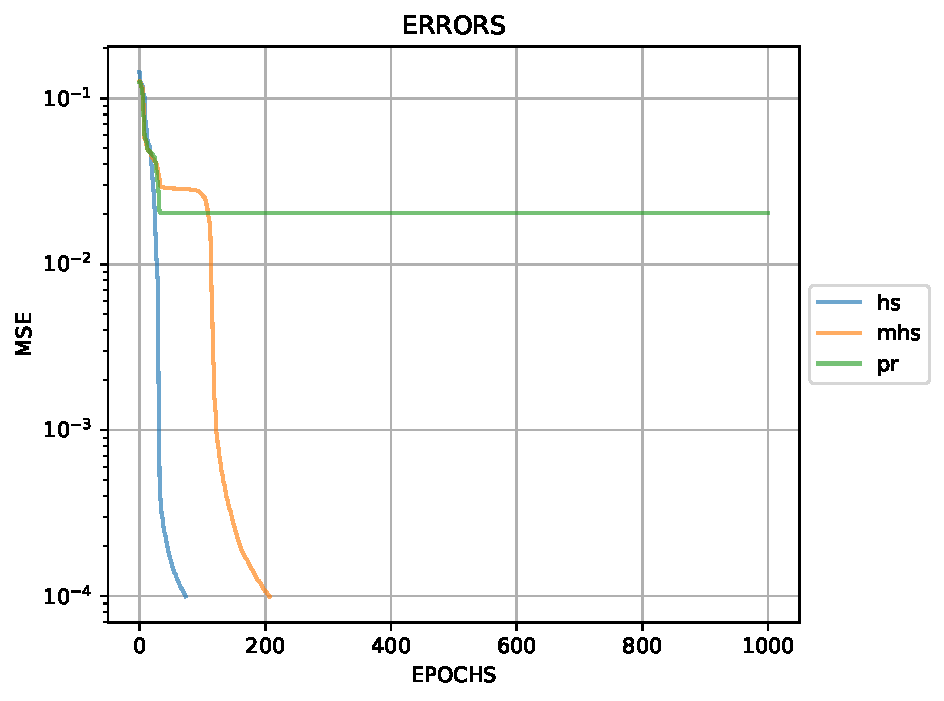
\includegraphics{img/comparisons/1_mse_beta_max_epochs_1000.pdf}
                    }
                    \caption{}
                    \label{fig:monks_1_MSE_CGD}
                \end{subfigure}
                \begin{subfigure}{0.4\textwidth}
                    \resizebox{\textwidth}{!}{
                        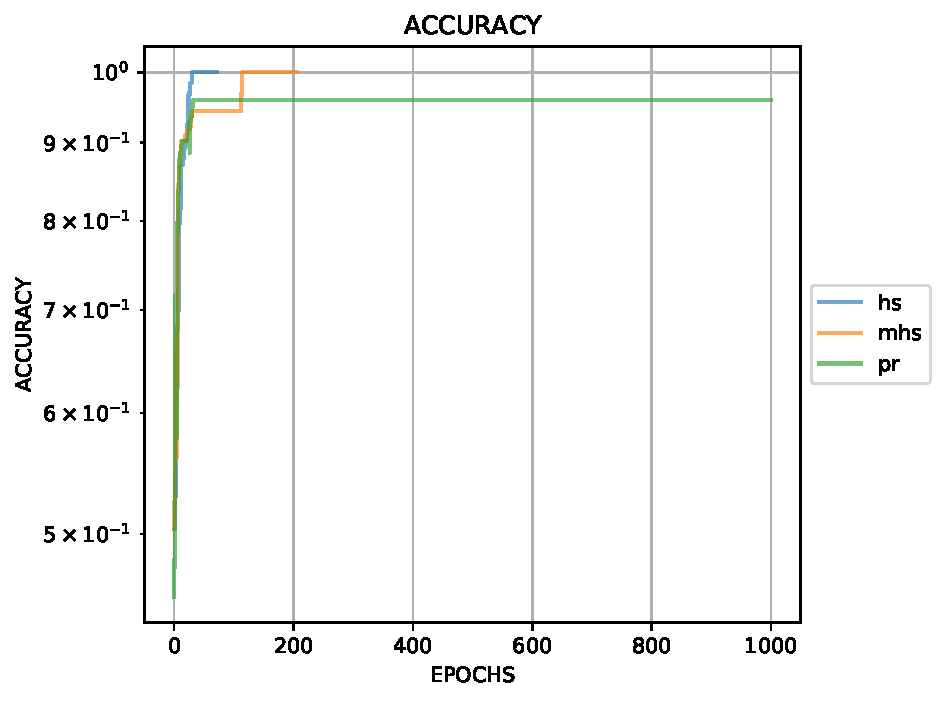
\includegraphics{img/comparisons/1_accuracy_beta_max_epochs_1000.pdf}
                    }
                    \caption{}
                    \label{fig:monks_1_ACC_CGD}
                \end{subfigure}
                \begin{subfigure}{0.4\textwidth}
                    \resizebox{\textwidth}{!}{
                        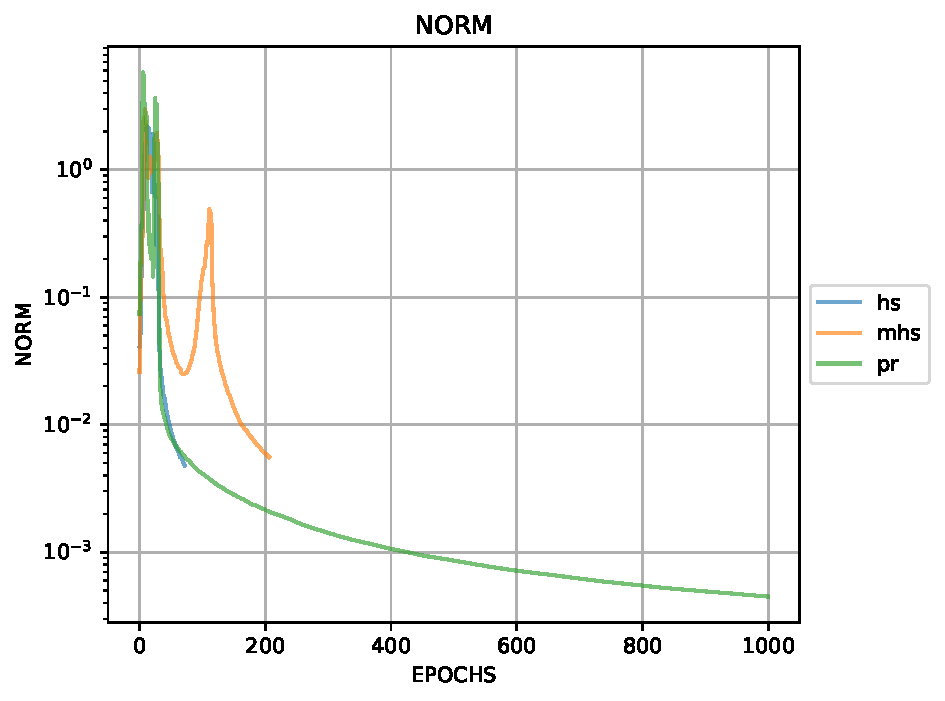
\includegraphics{img/comparisons/1_norm_beta_max_epochs_1000.pdf}
                    }
                    \caption{}
                    \label{fig:monks_1_NORM_CGD}
                \end{subfigure}
                \caption{Example of a final learning, accuracy score and convergence of norm curve on MONKS 1 with different beta methods.}
                \label{fig:monks_1_CGD}
            \end{figure}

             \begin{figure}[H]
                \centering
                \begin{subfigure}{0.40\textwidth}
                    \resizebox{\textwidth}{!}{
                        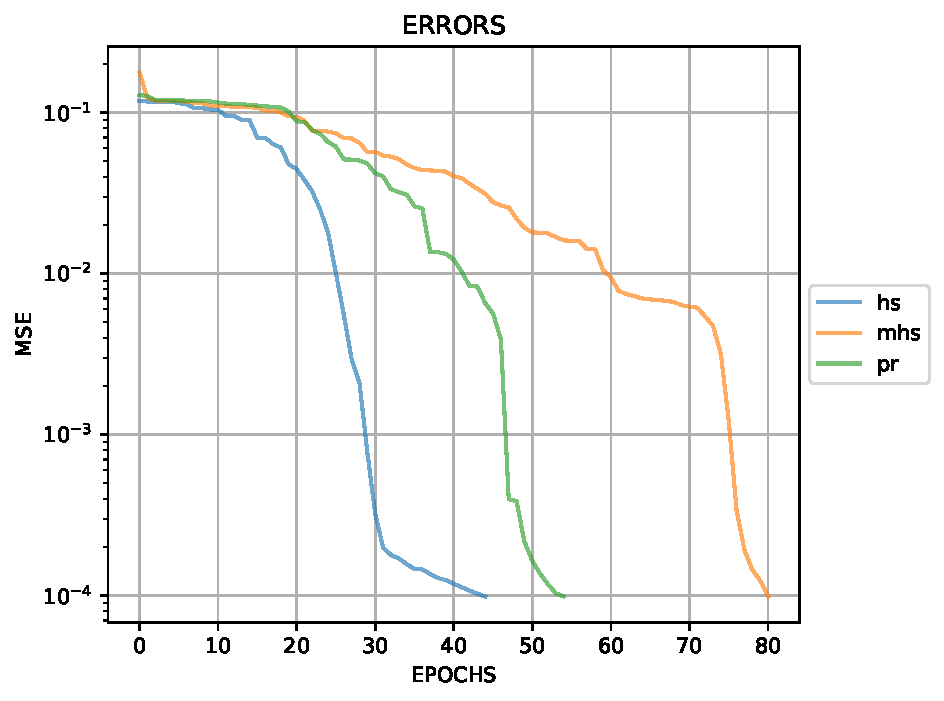
\includegraphics{img/comparisons/2_mse_beta_max_epochs_1000.pdf}
                    }
                    \caption{}
                    \label{fig:monks_2_MSE_CGD}
                \end{subfigure}
                \begin{subfigure}{0.40\textwidth}
                    \resizebox{\textwidth}{!}{
                        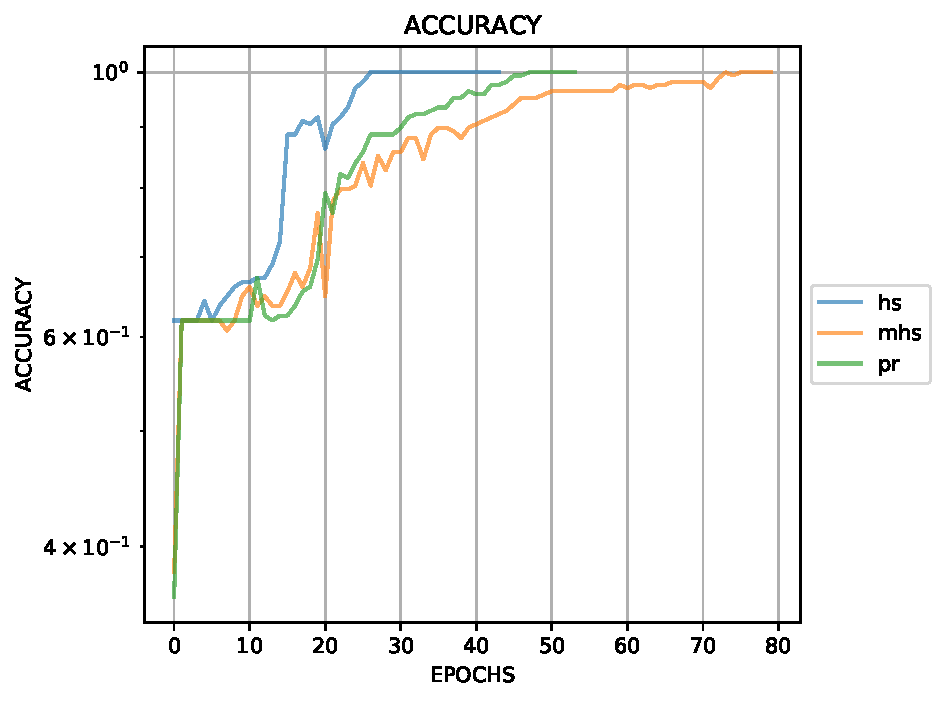
\includegraphics{img/comparisons/2_accuracy_beta_max_epochs_1000.pdf}
                    }
                    \caption{}
                    \label{fig:monks_2_ACC_CGD}
                \end{subfigure}
                \begin{subfigure}{0.40\textwidth}
                    \resizebox{\textwidth}{!}{
                        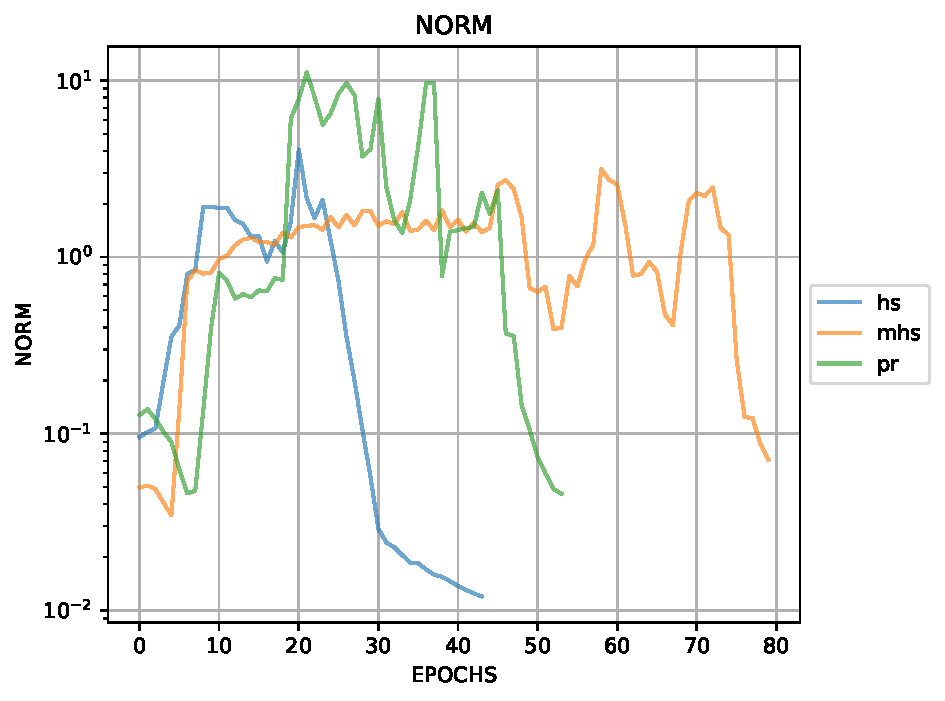
\includegraphics{img/comparisons/2_norm_beta_max_epochs_1000.pdf}
                    }
                    \caption{}
                    \label{fig:monks_2_NORM_CGD}
                \end{subfigure}
                \caption{Example of a final learning, accuracy score and convergence of norm curve on MONKS 2 with different beta methods.}
                \label{fig:monks_2_CGD}
            \end{figure}

            \begin{figure}[H]
                \centering
                \begin{subfigure}{0.40\textwidth}
                    \resizebox{\textwidth}{!}{
                        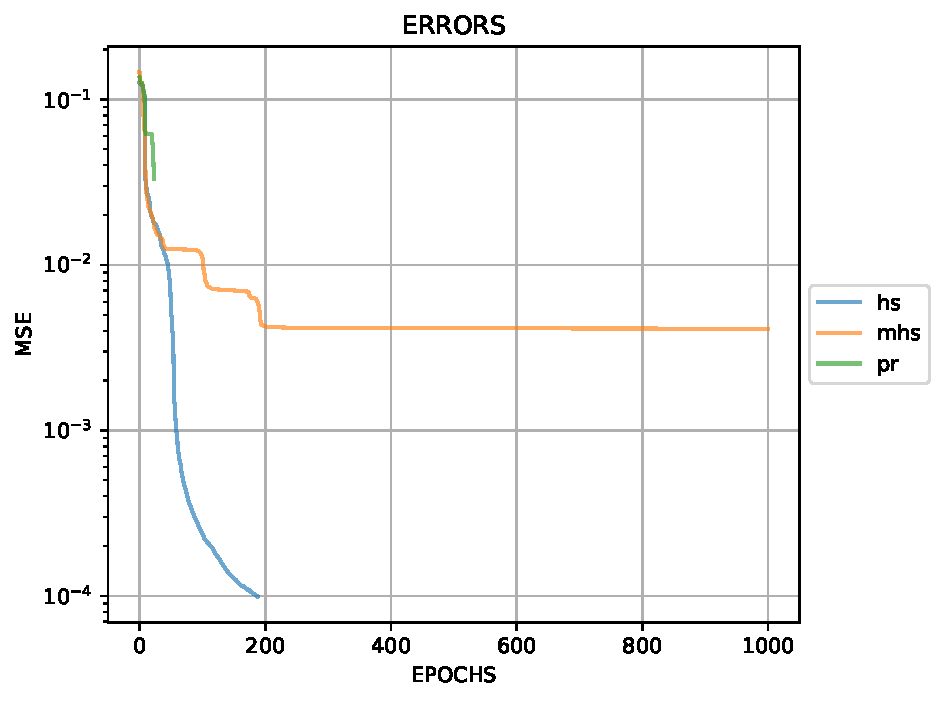
\includegraphics{img/comparisons/3_mse_beta_max_epochs_1000.pdf}
                    }
                    \caption{}
                    \label{fig:monks_3_MSE_CGD}
                \end{subfigure}
                \begin{subfigure}{0.40\textwidth}
                    \resizebox{\textwidth}{!}{
                        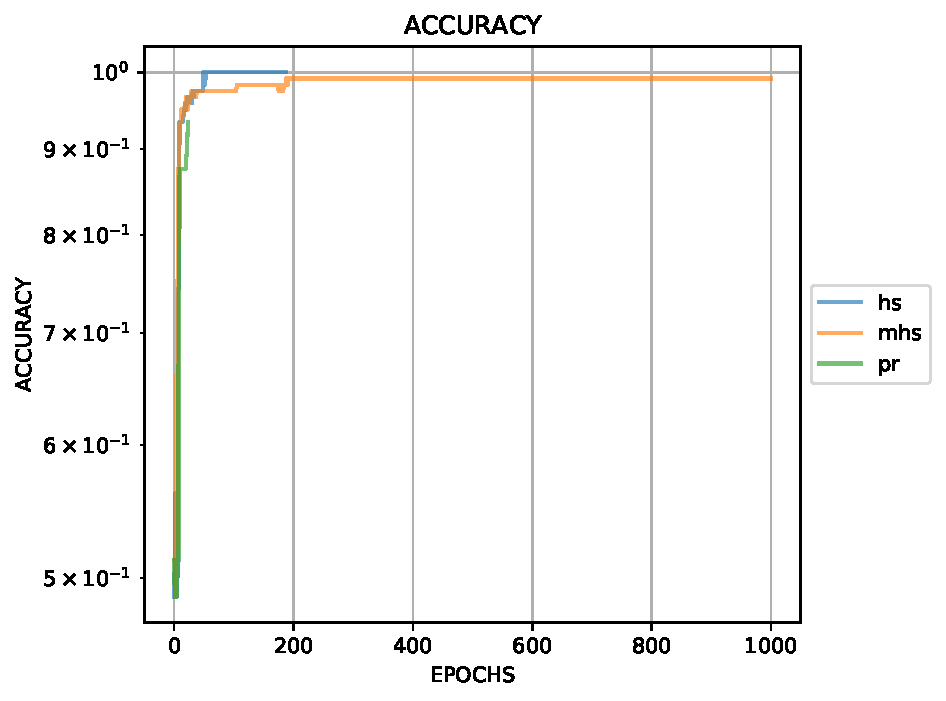
\includegraphics{img/comparisons/3_accuracy_beta_max_epochs_1000.pdf}
                    }
                    \caption{}
                    \label{fig:monks_3_ACC_CGD}
                \end{subfigure}
                \begin{subfigure}{0.40\textwidth}
                    \resizebox{\textwidth}{!}{
                        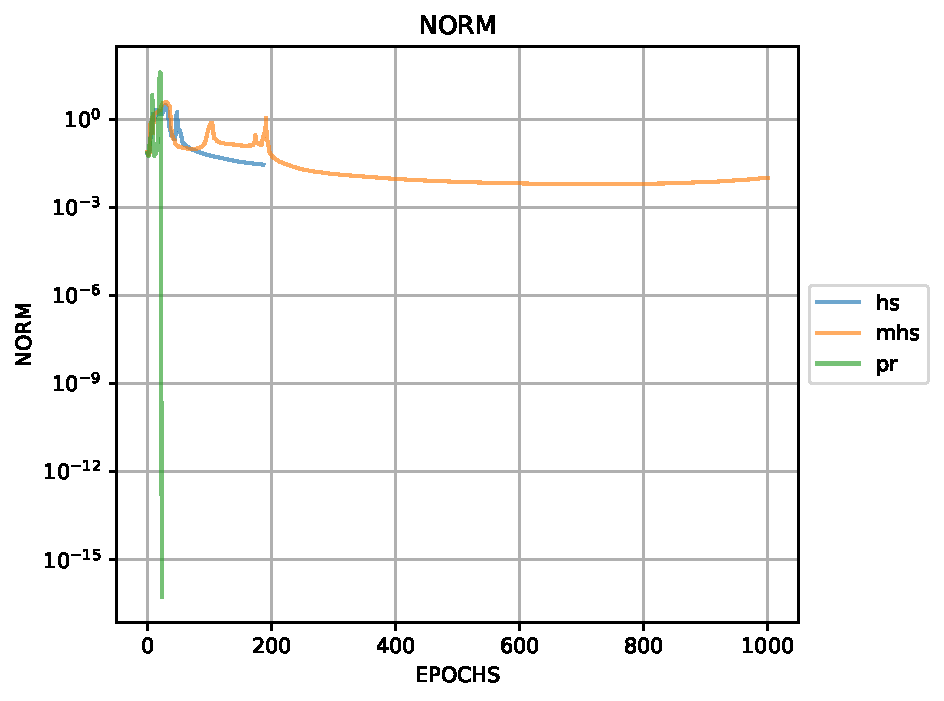
\includegraphics{img/comparisons/3_norm_beta_max_epochs_1000.pdf}
                    }
                    \caption{}
                    \label{fig:monks_3_NORM_CGD}
                \end{subfigure}
                \caption{Example of a final learning, accuracy score and convergence of norm curve on MONKS 3 with different beta methods.}
                \label{fig:monks_3_CGD}
            \end{figure}

            % subsection pr (end)

        % section conjugate_gradient_methods (end)

    % chapter monks_learning_curves (end)

    \chapter{CUP's learning curves} % (fold)
    \label{cha:cup_learning_curves}
        As in the previous section, the following curves are the result of the final tests on the test dataset. It has been plotted one of the 10 trails we used for building the statistics we presented in Section \ref{sec:cup}, hence each plot presents a possible learning curve for each dataset.

        \section{Stochastic Gradient Descent} % (fold)
        \label{sec:cup_sgd}

        \begin{figure}[H]
                \centering
                \begin{subfigure}{0.40\textwidth}
                    \resizebox{\textwidth}{!}{
                        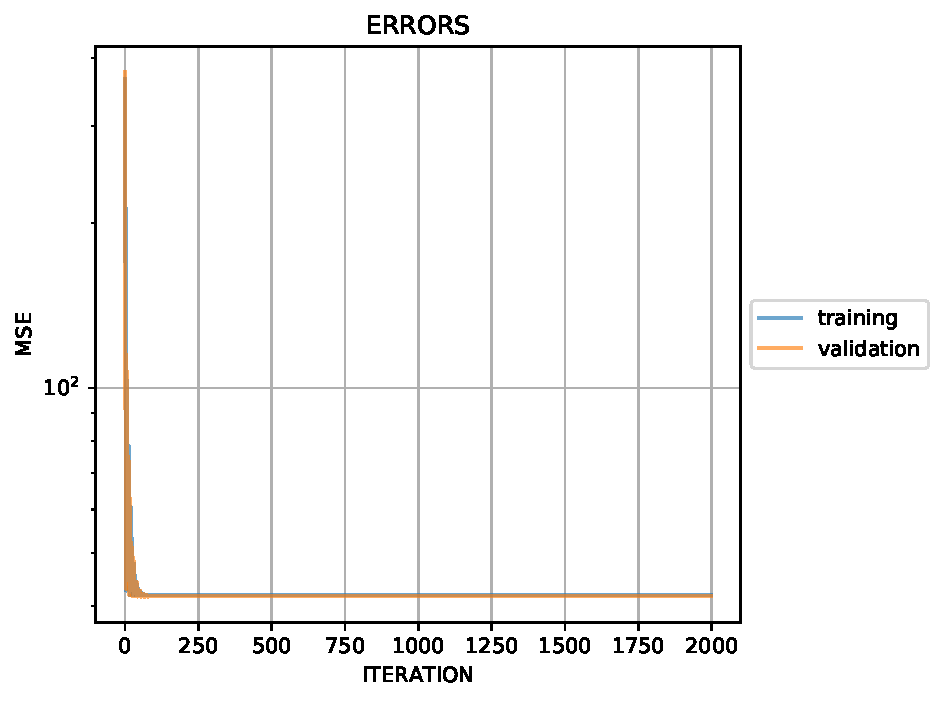
\includegraphics{img/analytics/CUP/CUP_mse_std.pdf}
                    }
                    \caption{}
                    \label{fig:CUP_MSE_CGD}
                \end{subfigure}
                \begin{subfigure}{0.40\textwidth}
                    \resizebox{\textwidth}{!}{
                        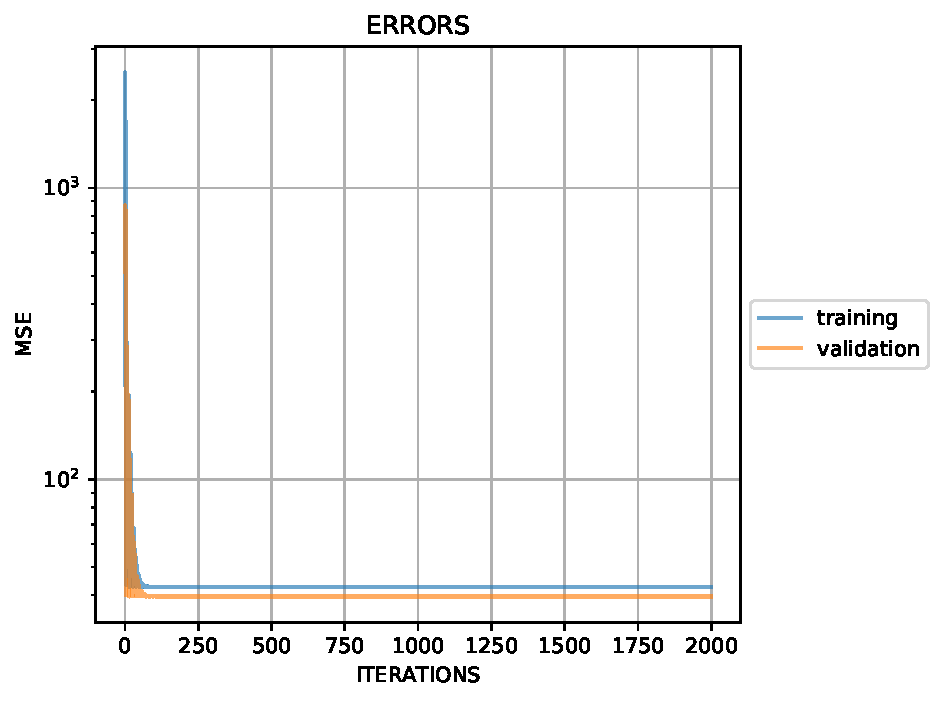
\includegraphics{img/analytics/CUP/CUP_mse_nesterov.pdf}
                    }
                    \caption{}
                    \label{fig:CUP_nest_CGD}
                \end{subfigure}
                \caption{Example of a training and validation errors for standard momentum, in Fig.\ref{fig:CUP_MSE_CGD} and nesterov momentum in Fig \ref{fig:CUP_nest_CGD}.}
                \label{fig:CUP_SGD}
            \end{figure}


        \section{Conjugate Gradient Methods} % (fold)
        \label{sec:conjugate_gradient_methods}
        
        \begin{figure}[H]
                \centering
                \begin{subfigure}{0.40\textwidth}
                    \resizebox{\textwidth}{!}{
                        \includegraphics{img/analytics/CUP/CUP_mse_mhs.pdf}
                    }
                    \caption{}
                    \label{fig:CUP_MSE_mhs}
                \end{subfigure}
                \begin{subfigure}{0.40\textwidth}
                    \resizebox{\textwidth}{!}{
                        \includegraphics{img/analytics/CUP/CUP_mse_hs.pdf}
                    }
                    \caption{}
                    \label{fig:CUP_MSE_hs}
                \end{subfigure}
                \begin{subfigure}{0.40\textwidth}
                    \resizebox{\textwidth}{!}{
                        \includegraphics{img/analytics/CUP/CUP_mse_pr.pdf}
                    }
                    \caption{}
                    \label{fig:CUP_MSE_pr}
                \end{subfigure}
                \caption{Example of a training and validation errors for $MHS^+$ in Fig.\ref{fig:CUP_MSE_mhs}, $HS^+$ in Fig.\ref{fig:CUP_MSE_hs} and $PR^+$ in Fig. \ref{fig:CUP_MSE_pr}.}
                \label{fig:cup_CGD}
            \end{figure}


\end{appendices}
